\documentclass{beamer}
\usepackage[export]{adjustbox}
\usepackage[frenchb]{babel}
\usepackage[T1]{fontenc}
\usepackage[utf8]{inputenc}
\usetheme{Warsaw}

\title[BT, BLE, BlueZ]{Bluetooth et BLE : Support dans Linux}
\author{maxime.chevallier@openwide.fr}
\date{09 février 2016}
\institute{Open Wide Ingénierie}
\begin{document}

% Afficher plan à chaque section
\AtBeginSection[]{
	\begin{frame}
		\tableofcontents[currentsection, hideothersubsections]
	\end{frame}
}

\setbeamertemplate{caption}{\raggedright\insertcaption\par}
\setbeamerfont{caption}{size=\tiny}
    \begin{frame}

	\titlepage

    \end{frame}

\begin{frame}
Intro
\end{frame}

\begin{frame}
\tableofcontents
\end{frame}

\section{Bluetooth}
\subsection{Présentation}
\begin{frame}
	\begin{minipage}[t]{0.25\linewidth}
		\uncover<2->{
			\begin{figure}
				
\includegraphics[height=2.5cm]{bt_logo.png}
				\caption{Logo Bluetooth}
			\end{figure}
		}
	\end{minipage}\hfill
	\begin{minipage}[t]{0.72\linewidth}
		\uncover<1->{
			\begin{block}{Historique}
				\begin{itemize}
					\item 1994 : Création ( Ericsson )
					\item 1998 : SIG (Ericsson, Intel, Nokia, Toshiba)
					\item 1999 : v1.0
					\item 2010 : v4.0 Low Energy
					\item 2014 : v4.2
				\end{itemize}
			\end{block}
		}
		\uncover<3->{
			\begin{block}{Caractéristiques physiques}
				\begin{itemize}
					\item 2.4 GHz
					\item 10m ( class 2 )
					\item Max 24Mb/s
					\item 79 cannaux, AFH
					\item Conso : 1W
				\end{itemize}
			\end{block}
		}
	\end{minipage}
\end{frame}

% Présenter des schémas
\subsection{Architecture logique}

\begin{frame}
	\begin{minipage}[t]{0.45\linewidth}
	\uncover<1->{
		\begin{figure}
			\vspace{0.5cm}
			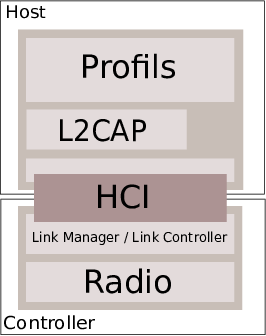
\includegraphics[height=5.5cm]{arch_core.png}
			\caption{Bluetooth core}
		\end{figure}
	}
	\end{minipage}
	\begin{minipage}[t]{0.52\linewidth}
		\uncover<2->{
		\begin{block}{Host}
			\begin{itemize}
				\item Logique Métier
				\item Scheduling
				\item Buffering
				\item QoS
			\end{itemize}
		\end{block}
		}
		\uncover<3->{
		\begin{block}{Controller}
			\begin{itemize}
				\item Connexion
				\item Découverte
				\item Sécurité
				\item QoS
			\end{itemize}
		\end{block}
		}
	\end{minipage}
\end{frame}

\begin{frame}
\begin{minipage}[t]{0.60\linewidth}
	\begin{figure}
		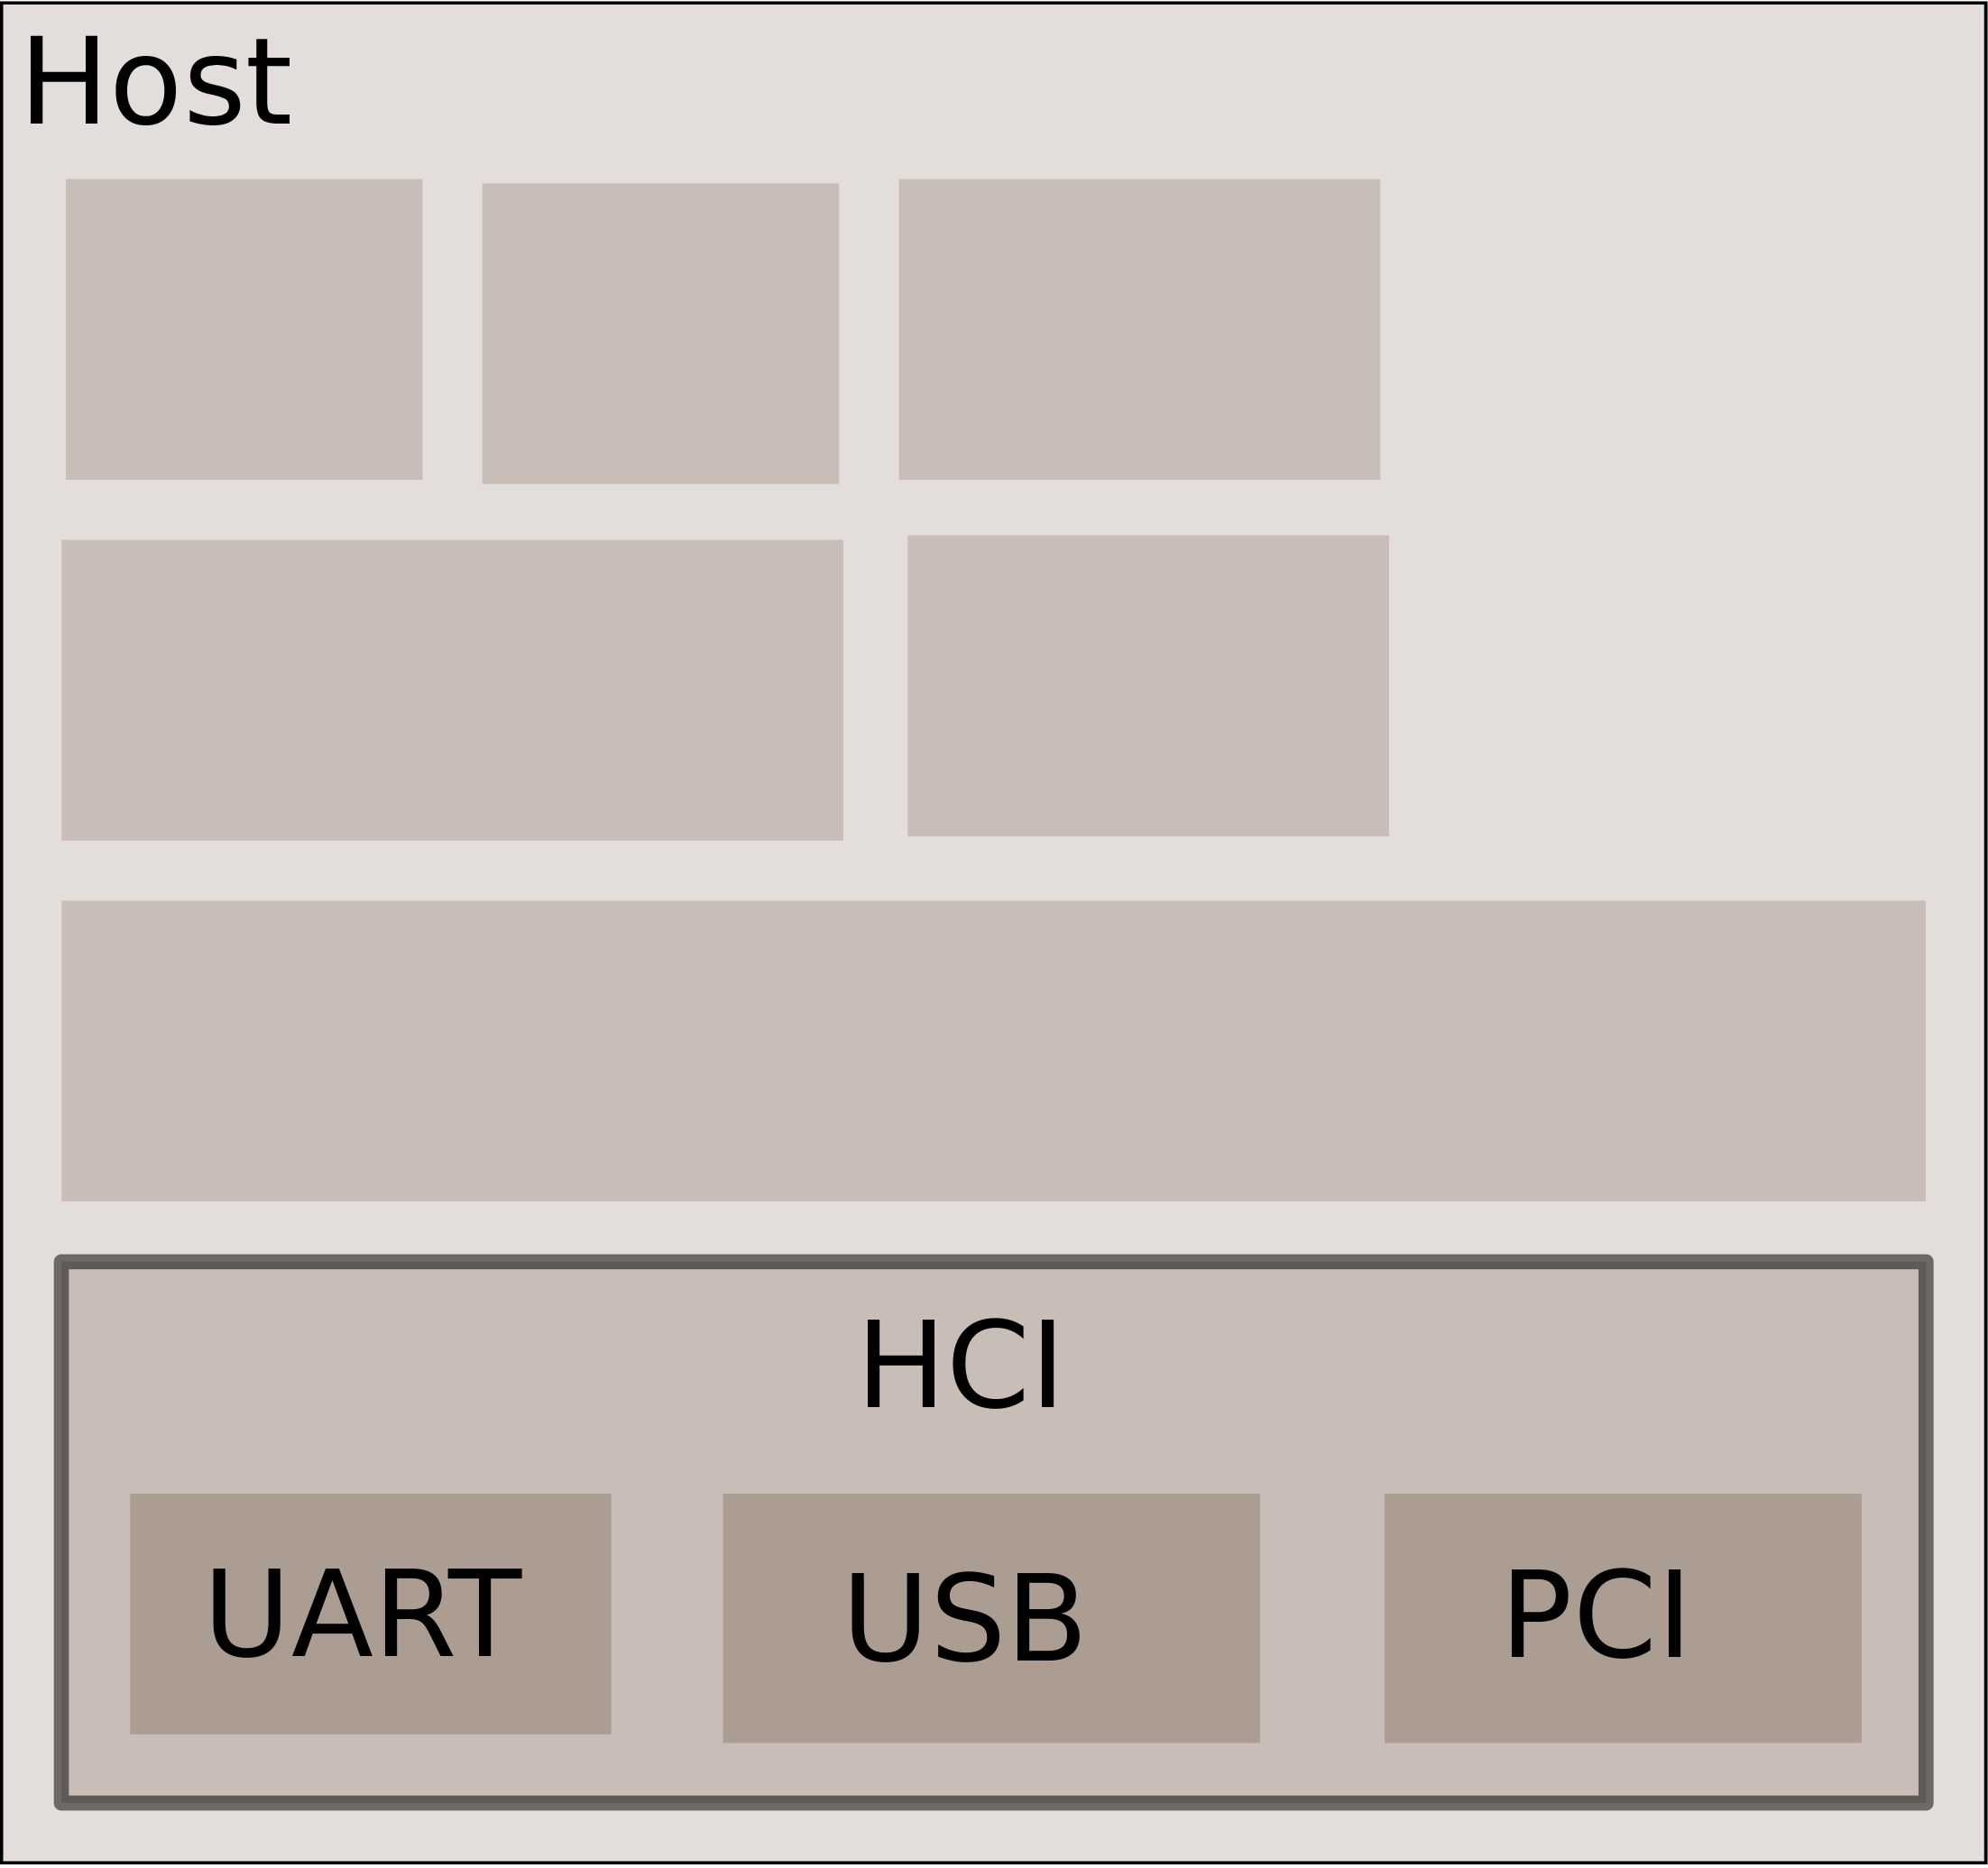
\includegraphics[height=5.5cm]{arch_log_hci.png}
		\caption{Host to Controller Interface}
	\end{figure}
\end{minipage}
\begin{minipage}[t]{0.30\linewidth}
	\begin{block}{HCI}
		\begin{itemize}
			\item Uniformisation
			\item Abstraction
		\end{itemize}
		Commandes : 
		\begin{itemize}
			\item Données
			\item Configuration
			\item Évènements
		\end{itemize}
	\end{block}
\end{minipage}
\end{frame}

\begin{frame}
	\begin{minipage}[t]{0.60\linewidth}
		\begin{figure}
			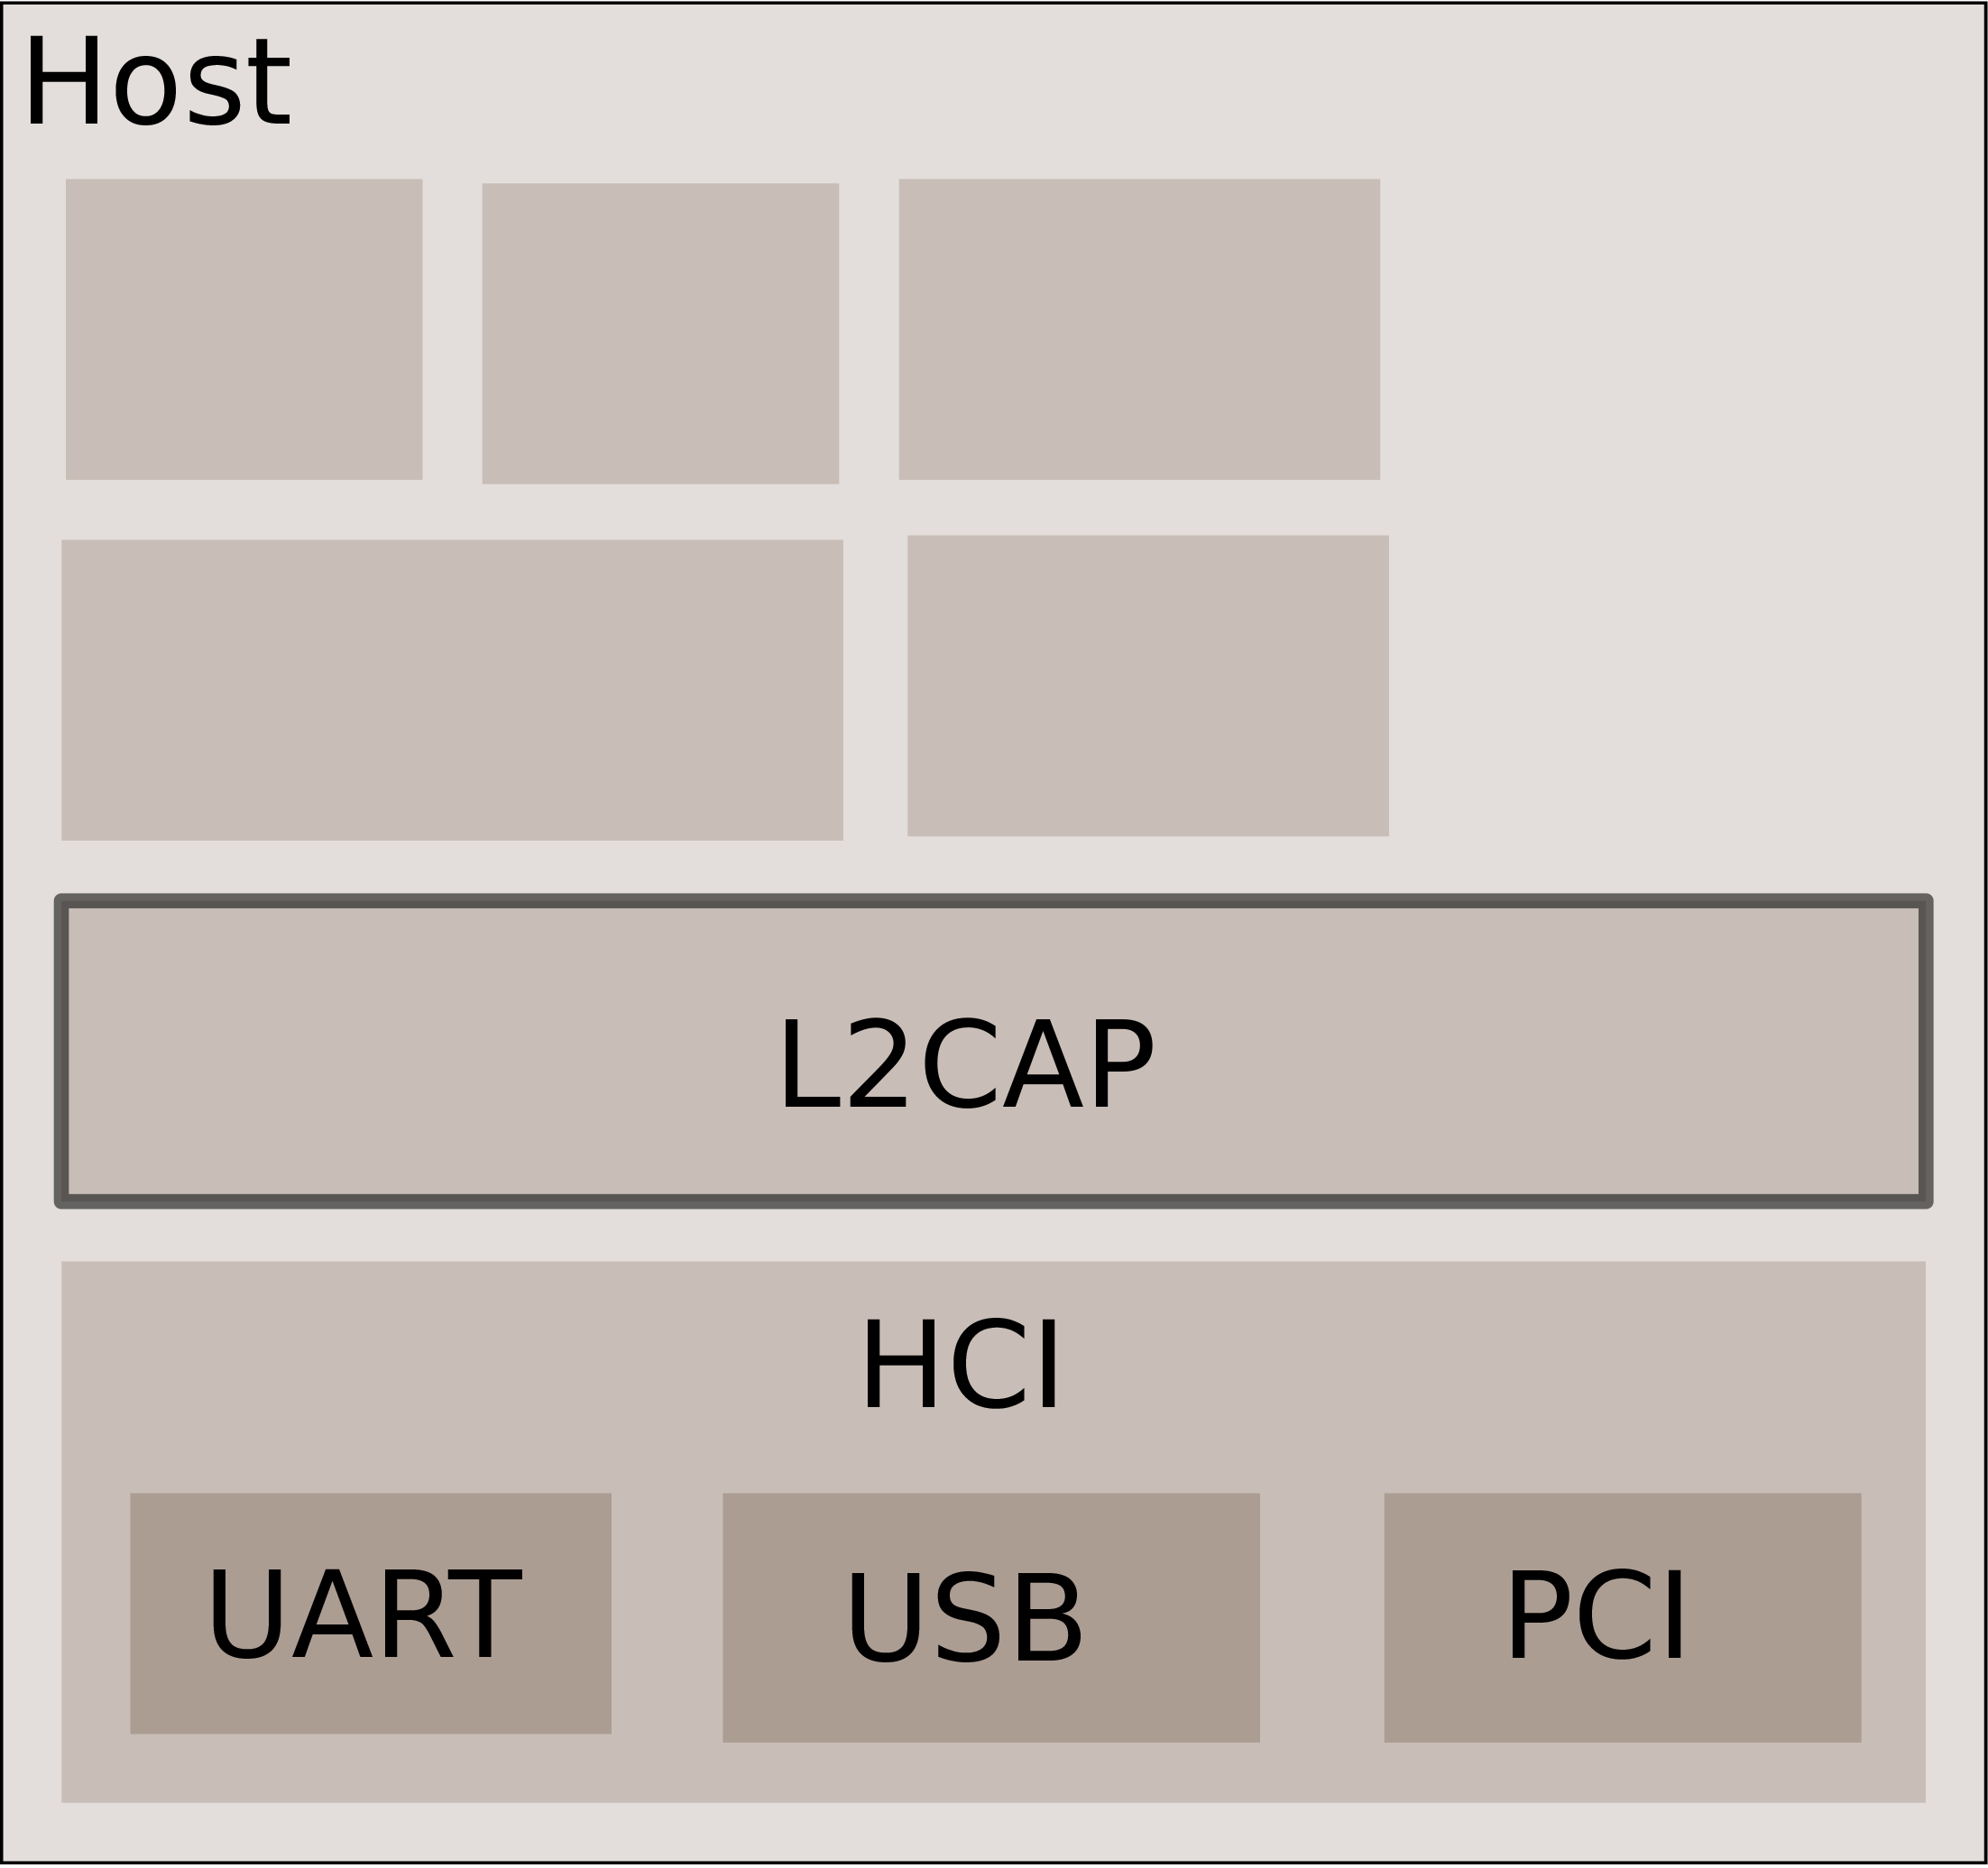
\includegraphics[height=5cm]{arch_log_l2cap.png}
			\caption{Logical Link Control and Adaptation Protocol}
		\end{figure}
	\end{minipage}
	\begin{minipage}[t]{0.30\linewidth}
		\begin{block}{L2CAP}
			Socle pour de nombreux profils :
			\begin{itemize}
				\item Multiplexage
				\item Buffering
				\item QoS
				\item Scheduling
			\end{itemize}
		\end{block}
	\end{minipage}
\end{frame}

\begin{frame}
	\begin{minipage}[t]{0.60\linewidth}
		\uncover<1->{
		\begin{figure}
			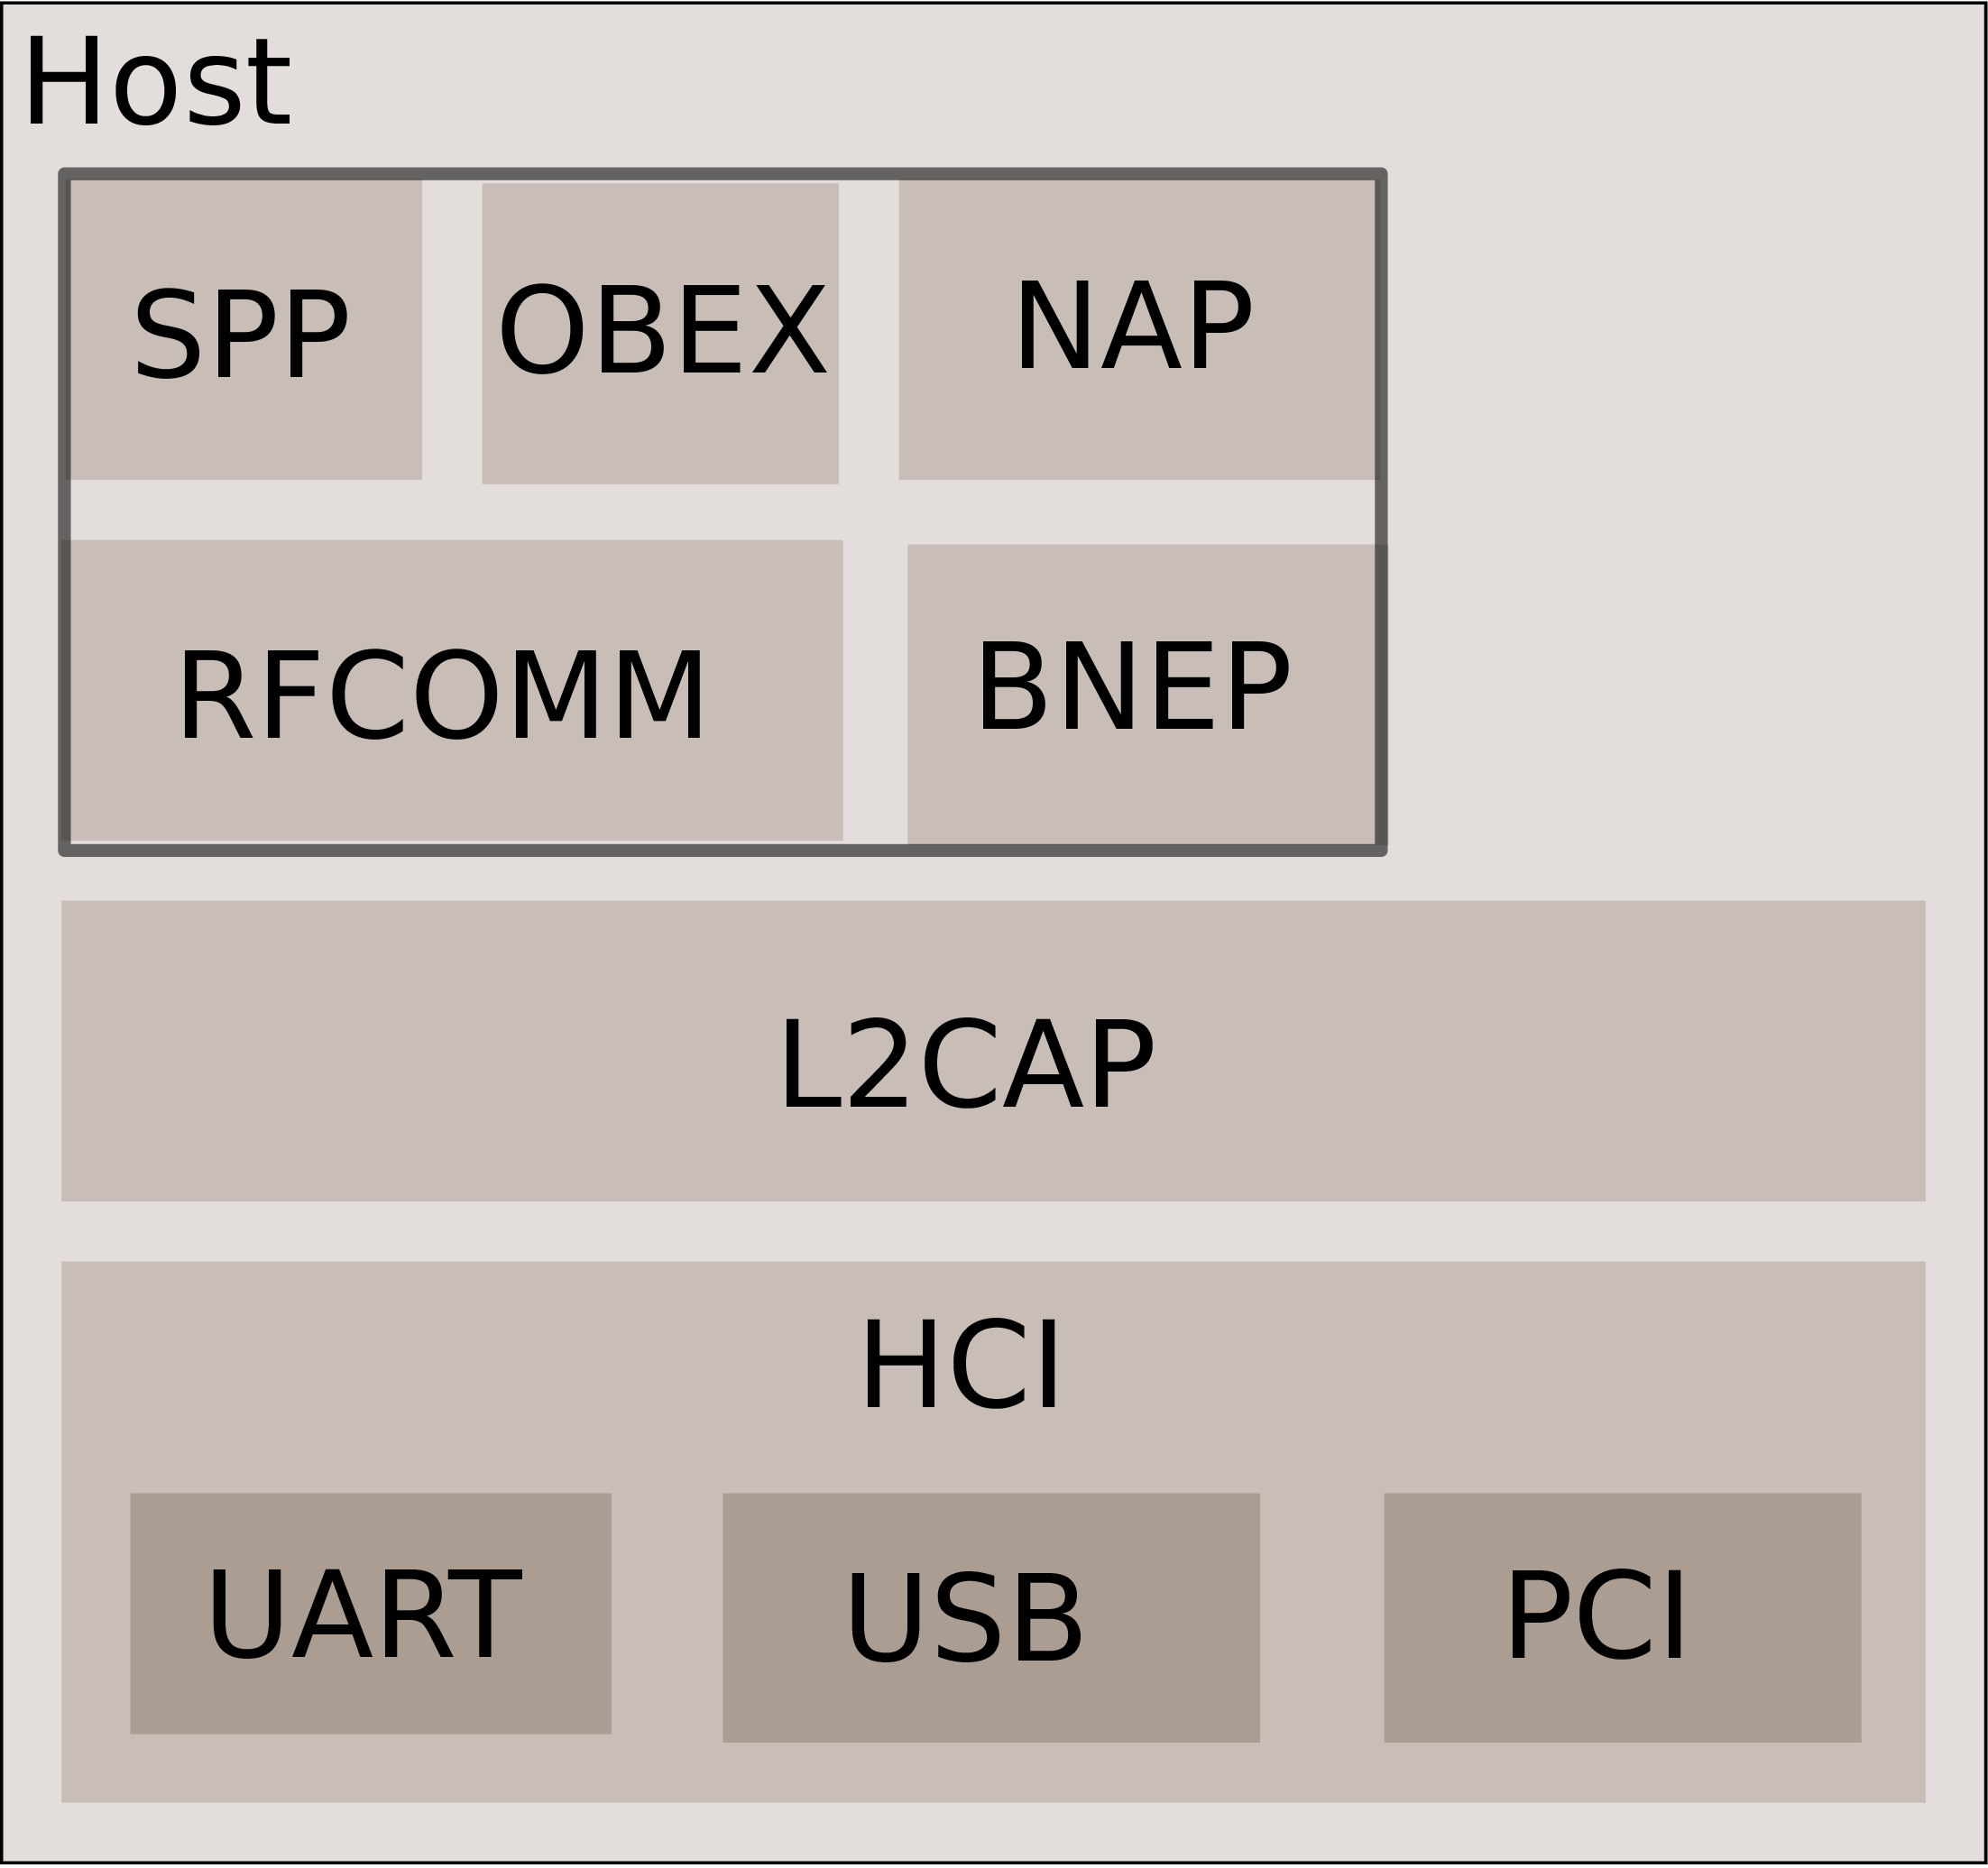
\includegraphics[height=5cm]{arch_log_all.png}
			\caption{Profils}
		\end{figure}
		}
	\end{minipage}
	\begin{minipage}[t]{0.38\linewidth}
		\uncover<2->{
		\begin{block}{Protocoles}
			\begin{itemize}
				\item RFCOMM
				\item BNEP
				\item AVCTP { \tiny( controle A/V )}
				\item AVDTP { \tiny ( transport  A/V )}
			\end{itemize}
		\end{block}
		}
		\uncover<3->{
		\begin{block}{Profils}
			{ \footnotesize
			\begin{itemize}
				\item Serial Port Profile
				\item Human Interface Device
				\item Personnal Area Network
				\item Phone Book Access Profile
			\end{itemize}
			}
		\end{block}
		}
	\end{minipage}
\end{frame}

\subsection{Appairage}
\begin{frame}
	\begin{minipage}[t]{0.45\linewidth}
		\uncover<1->{
		\begin{block}{Découverte}
			\begin{enumerate}
				\item Inquiry
				\item Paging
				\item Connexion
			\end{enumerate}
		\end{block}
		}
		\uncover<2->{
		\begin{block}{Appairage}
			\begin{itemize}
				\item Connexion automatique,
				\item sécurisée,
				\item authentifiée,
				\item adaptée à l'appareil.
			\end{itemize}
		\end{block}
		}
	\end{minipage}
	\begin{minipage}[t]{0.45\linewidth}
		\uncover<3->{
		\begin{figure}
		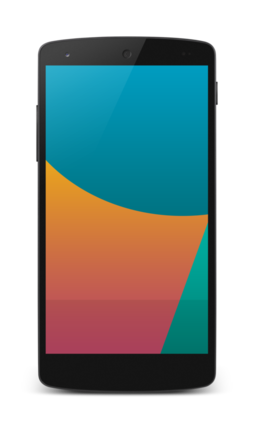
\includegraphics[height=2cm]{nex_5.png}
		\end{figure}
		}
		\uncover<4->{
		\begin{figure}
		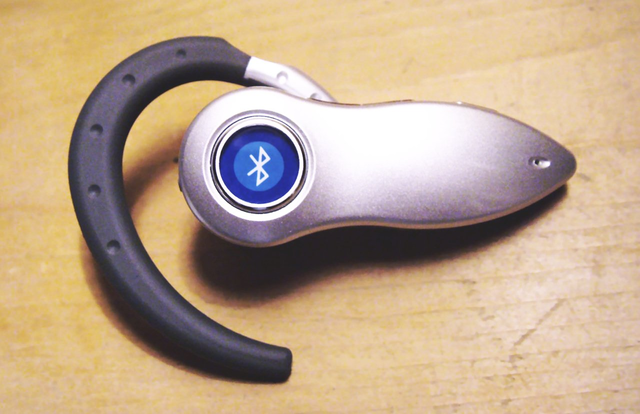
\includegraphics[height=1.5cm]{headset.png}
		\end{figure}
		}
		\uncover<5->{
		\begin{figure}
		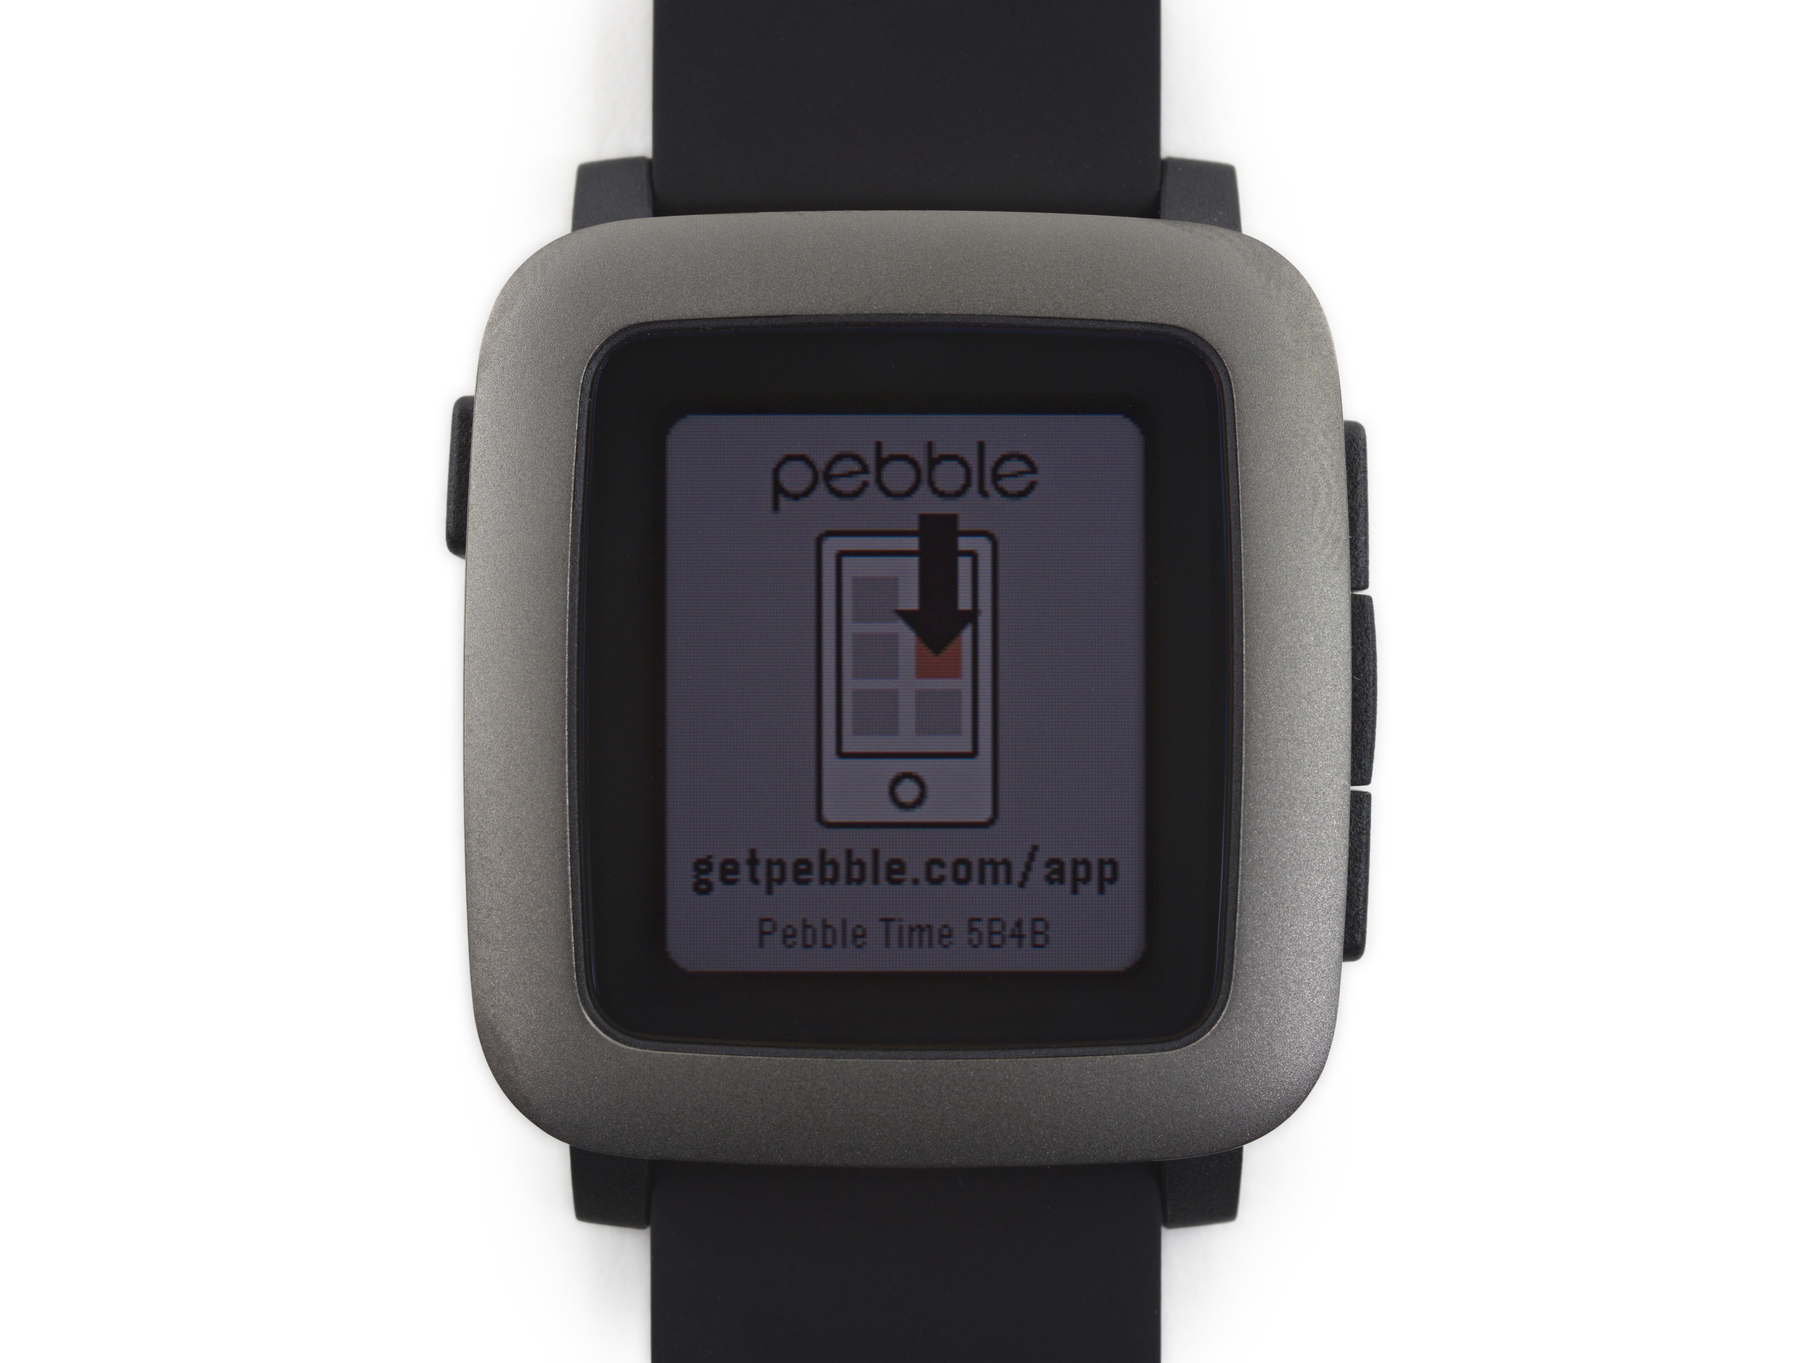
\includegraphics[height=1.5cm]{pt.jpg}
		\end{figure}
		}
	\end{minipage}
\end{frame}

\subsection{Découverte de services}
\begin{frame}
\begin{minipage}[t]{0.70\linewidth}

\begin{figure}
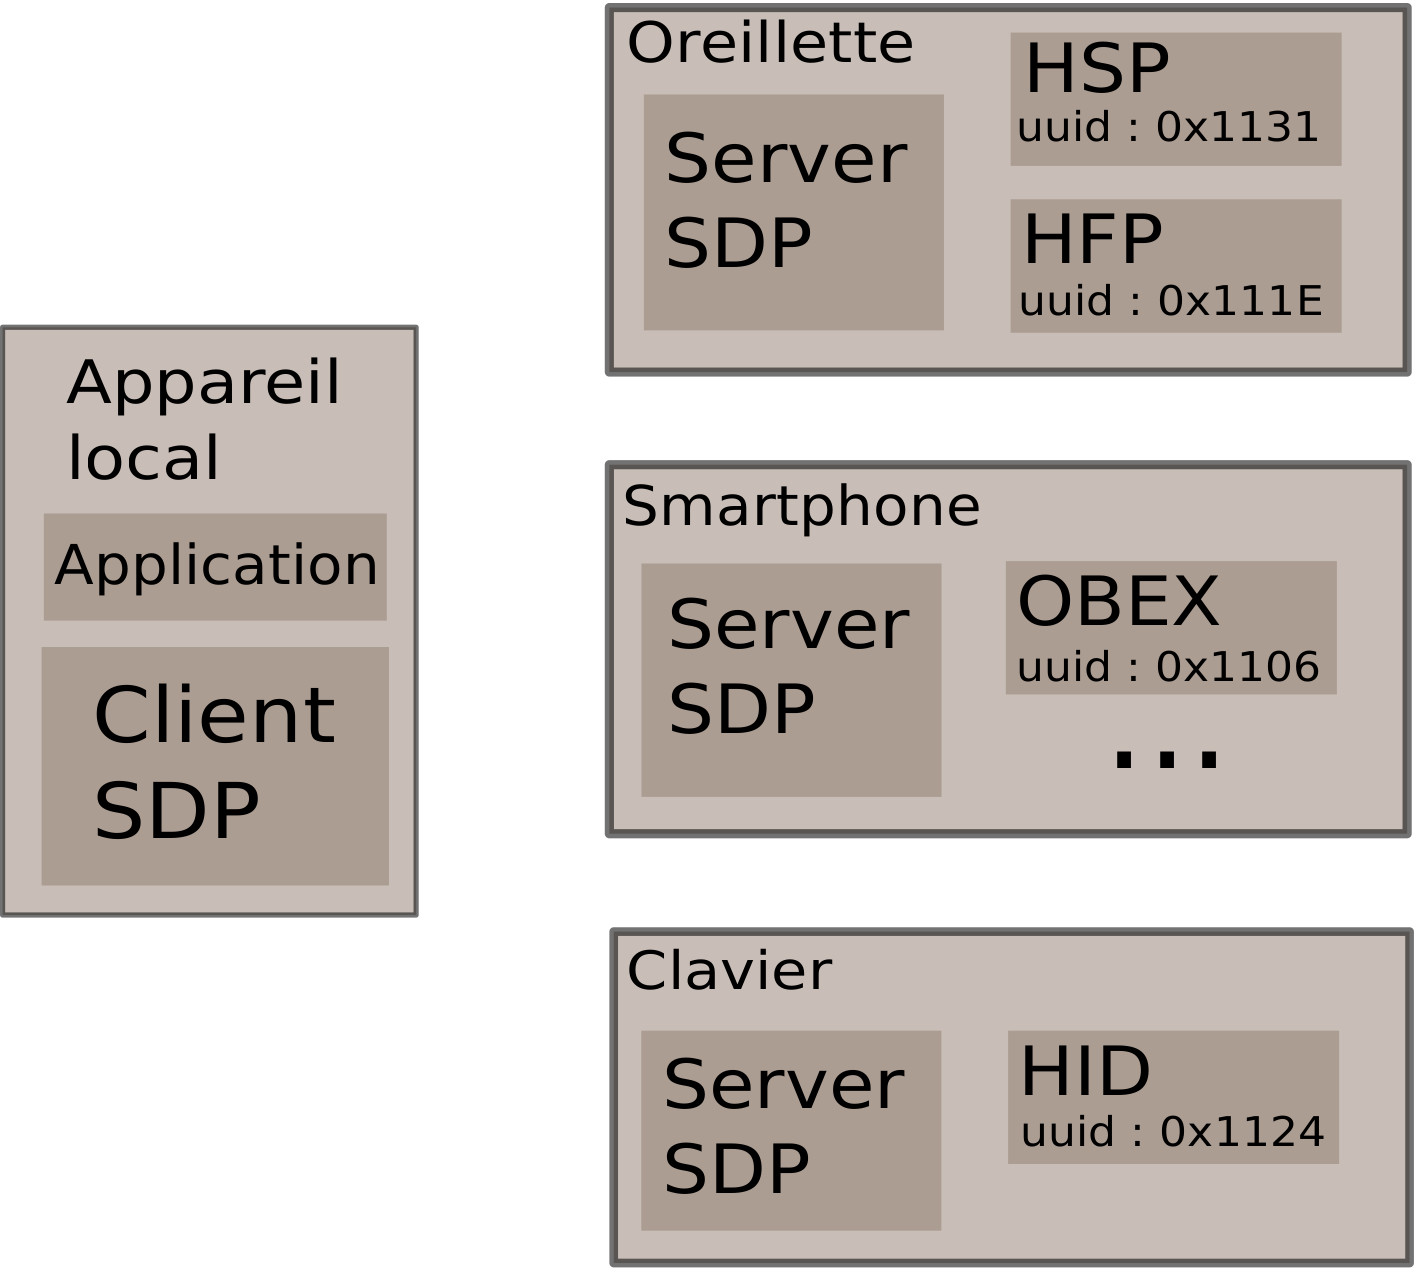
\includegraphics[height=5.5cm]{sdp.png}
\caption{Service Discovery Protocol}
\end{figure}


\end{minipage}
\begin{minipage}[t]{0.27\linewidth}
\begin{block}{UUID}
Identifient des :
\begin{itemize}
\item Profils
\item Protocoles
\item Attributs GATT
\end{itemize}
\end{block}

\end{minipage}
{\tiny Liste : https://www.bluetooth.com/specifications/assigned-numbers/service-discovery}
\end{frame}

\section{Bluetooth Low Energy}
\subsection{Présentation}
\begin{frame}
	\begin{minipage}[t]{0.45\linewidth}
	\uncover<2->{
		\begin{figure}
			
\includegraphics[height=3.25cm]{img/bt_logo_smart_and_ready.jpg}
			\caption{Logos Bluetooth Low Energy}
		\end{figure}
	}
	\end{minipage}
	\begin{minipage}[t]{0.52\linewidth}
		\uncover<1->{
		\begin{block}{Bluetooth Smart}
			\begin{itemize}
				\item 2006 : Wibree ( Nokia )
				\item 2010 : Bluetooth 4.0
			\end{itemize}
		\end{block}
		}
		\uncover<3->{
		\begin{block}{Caractéristiques}
			\begin{itemize}
				\item 2.4 GHz
				\item 40 cannaux
				\item 1 Mbit/s
				\item Conso entre 0.01W et 0.5W
			\end{itemize}
		\end{block}
		}
	\end{minipage}
\end{frame}

\subsection{Architecture logique}
\begin{frame}


\begin{minipage}[t]{0.47\linewidth}
	\begin{figure}
		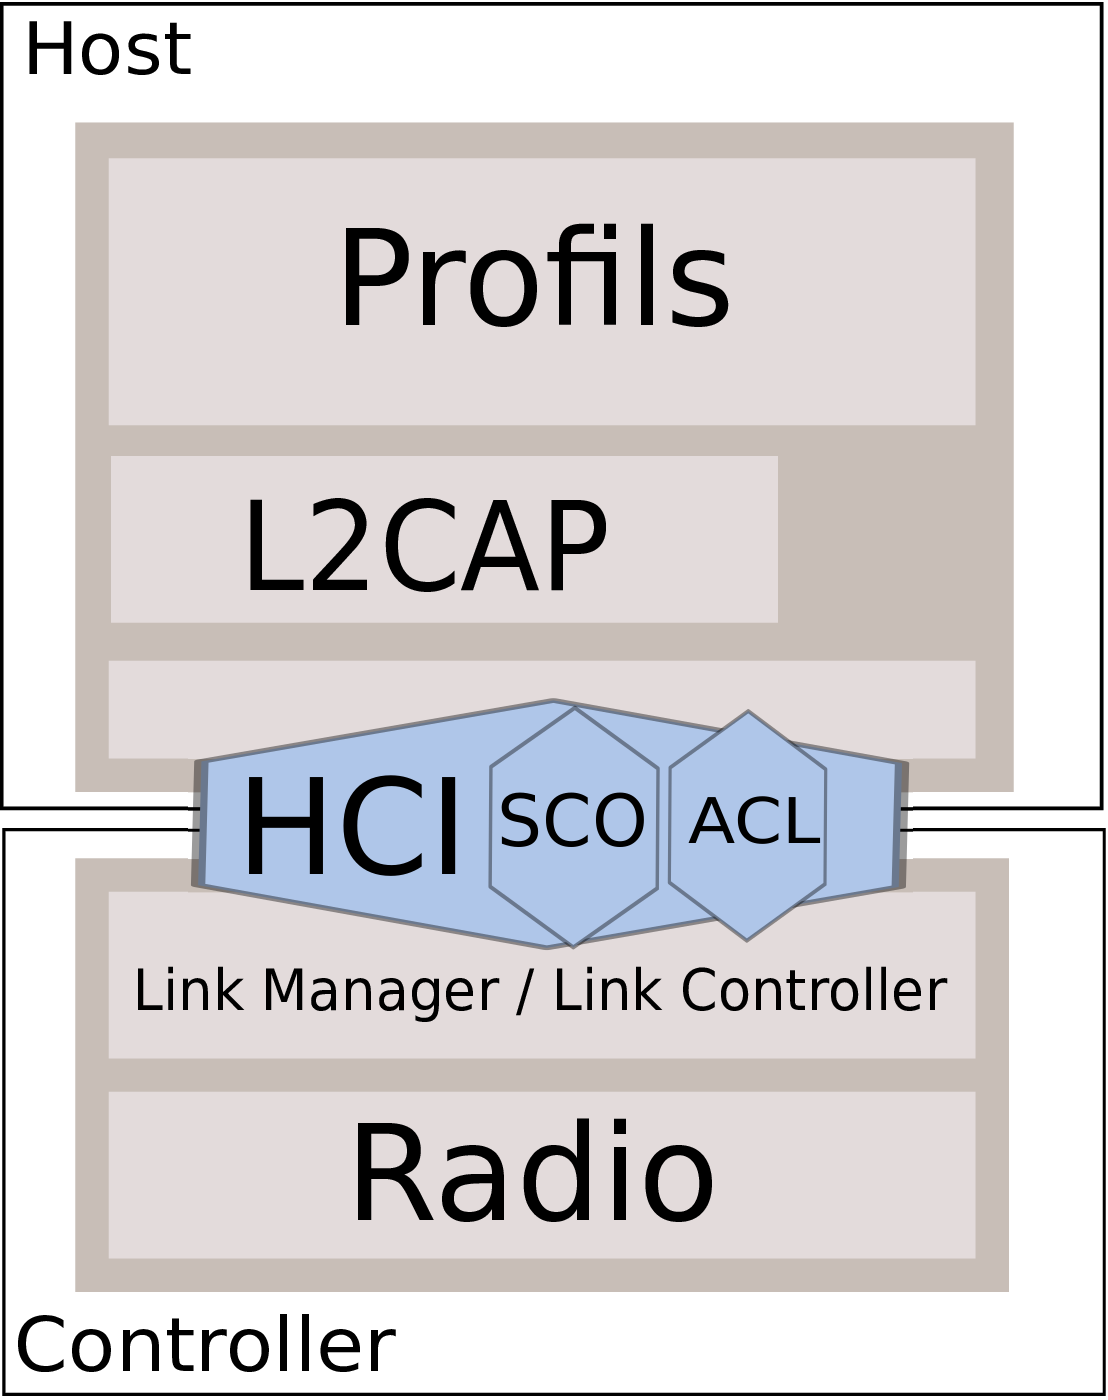
\includegraphics[height=6cm]{img/arch_core.png}
		\caption{Core BR/EDR}
	\end{figure}
\end{minipage}
\begin{minipage}[t]{0.45\linewidth}
	\begin{figure}
		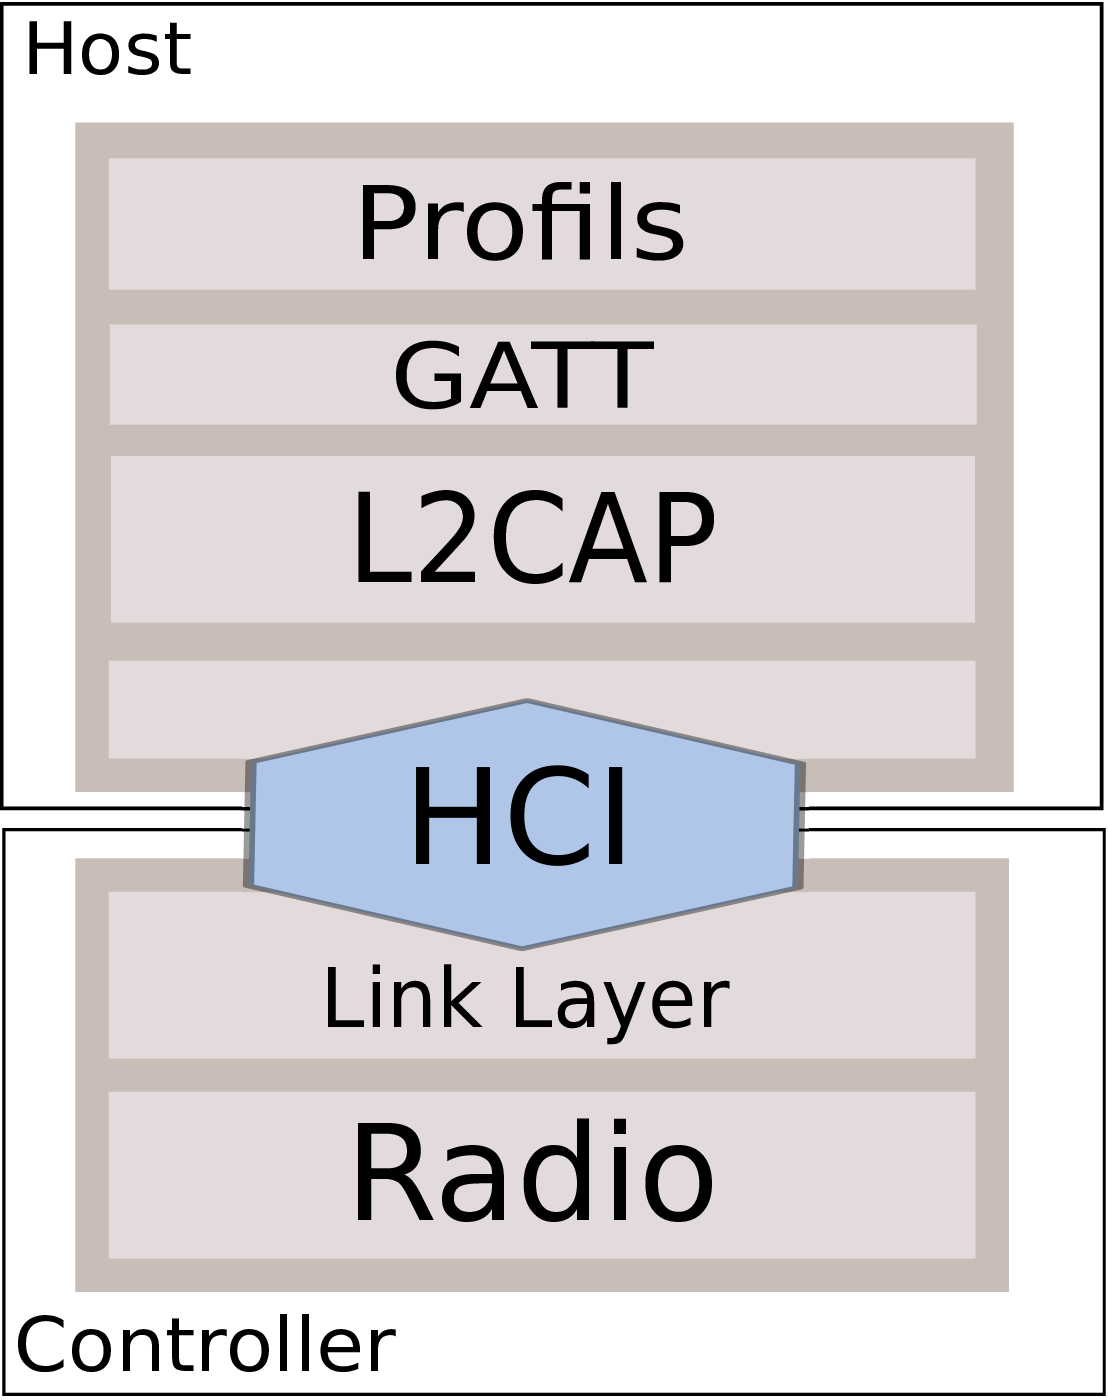
\includegraphics[height=6cm]{img/arch_core_ble.png}
		\caption{Core BLE}
	\end{figure}
\end{minipage}
% ici schema diff BT/BLE de bt.org
\end{frame}
\begin{frame}

\begin{minipage}[t]{0.47\linewidth}
	\begin{figure}
		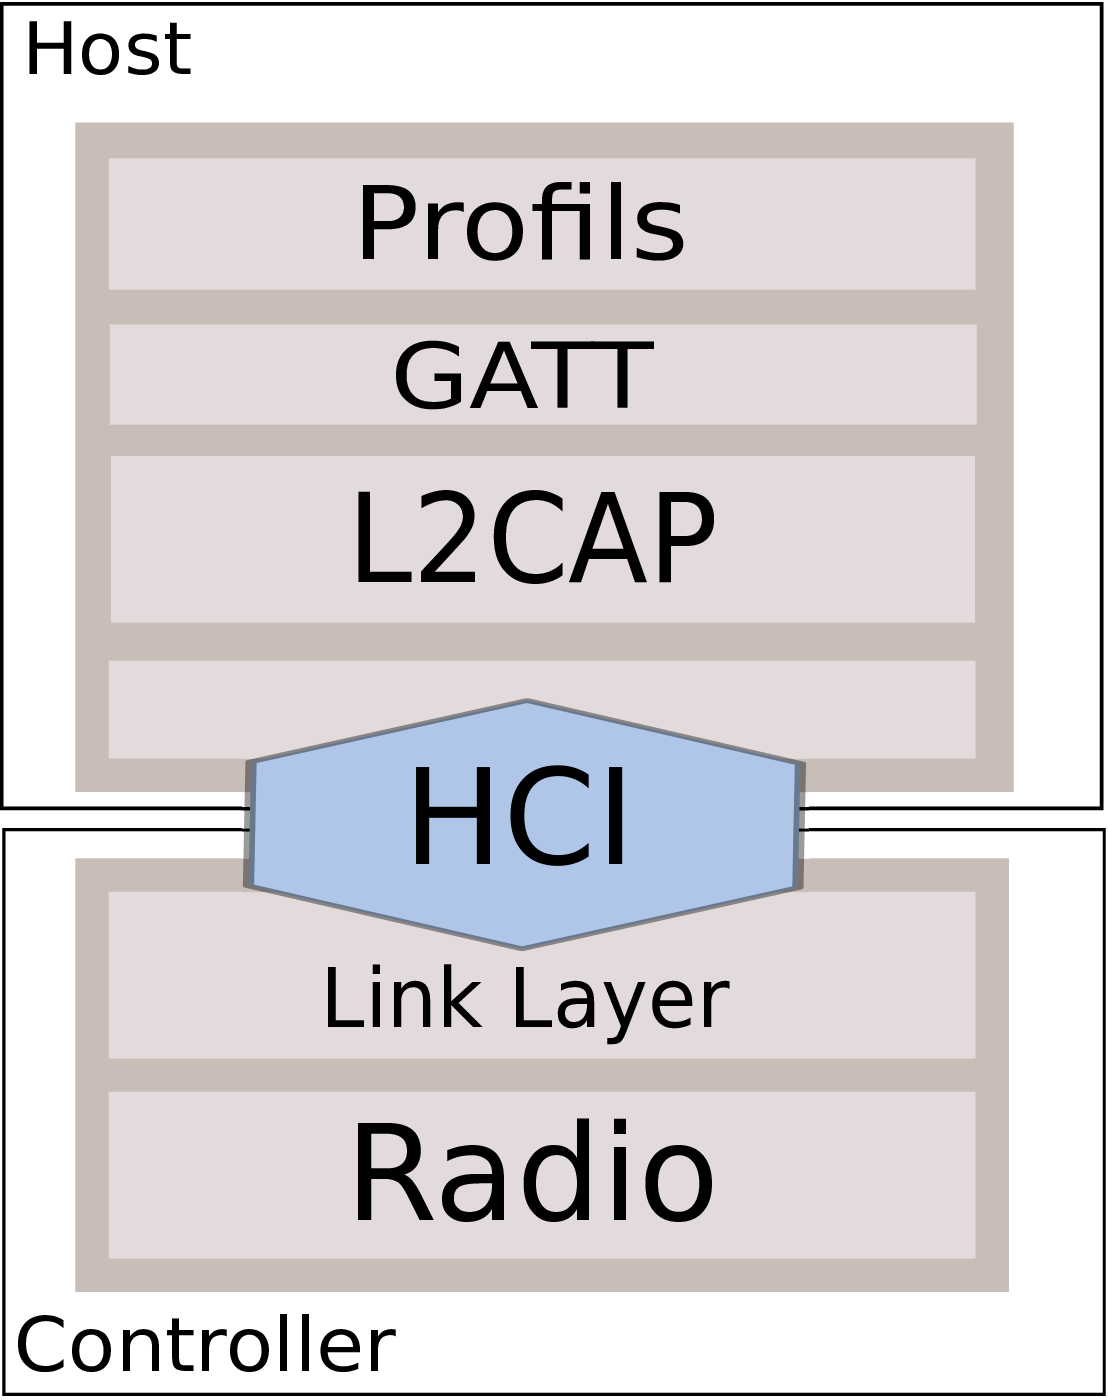
\includegraphics[height=6cm]{img/arch_core_ble.png}
		\caption{Core BLE}
	\end{figure}
\end{minipage}
\begin{minipage}[t]{0.45\linewidth}
	\begin{block}{Link Layer}
		\begin{itemize}
			\item Advertising
			\item Scanning
			\item Connected
		\end{itemize}
	\end{block}
	\begin{block}{Sécurité}
		\begin{itemize}
			\item Clé côté Host
			\item AES 128
			\item Adresses :
			\begin{itemize}
				\item Publique
				\item Aléatoire
			\end{itemize}
		\end{itemize}
	\end{block}
\end{minipage}
% ici schema diff BT/BLE de bt.org
\end{frame}

\begin{frame}
	\begin{minipage}[t]{0.60\linewidth}
		\uncover<1->{
			\begin{figure}
				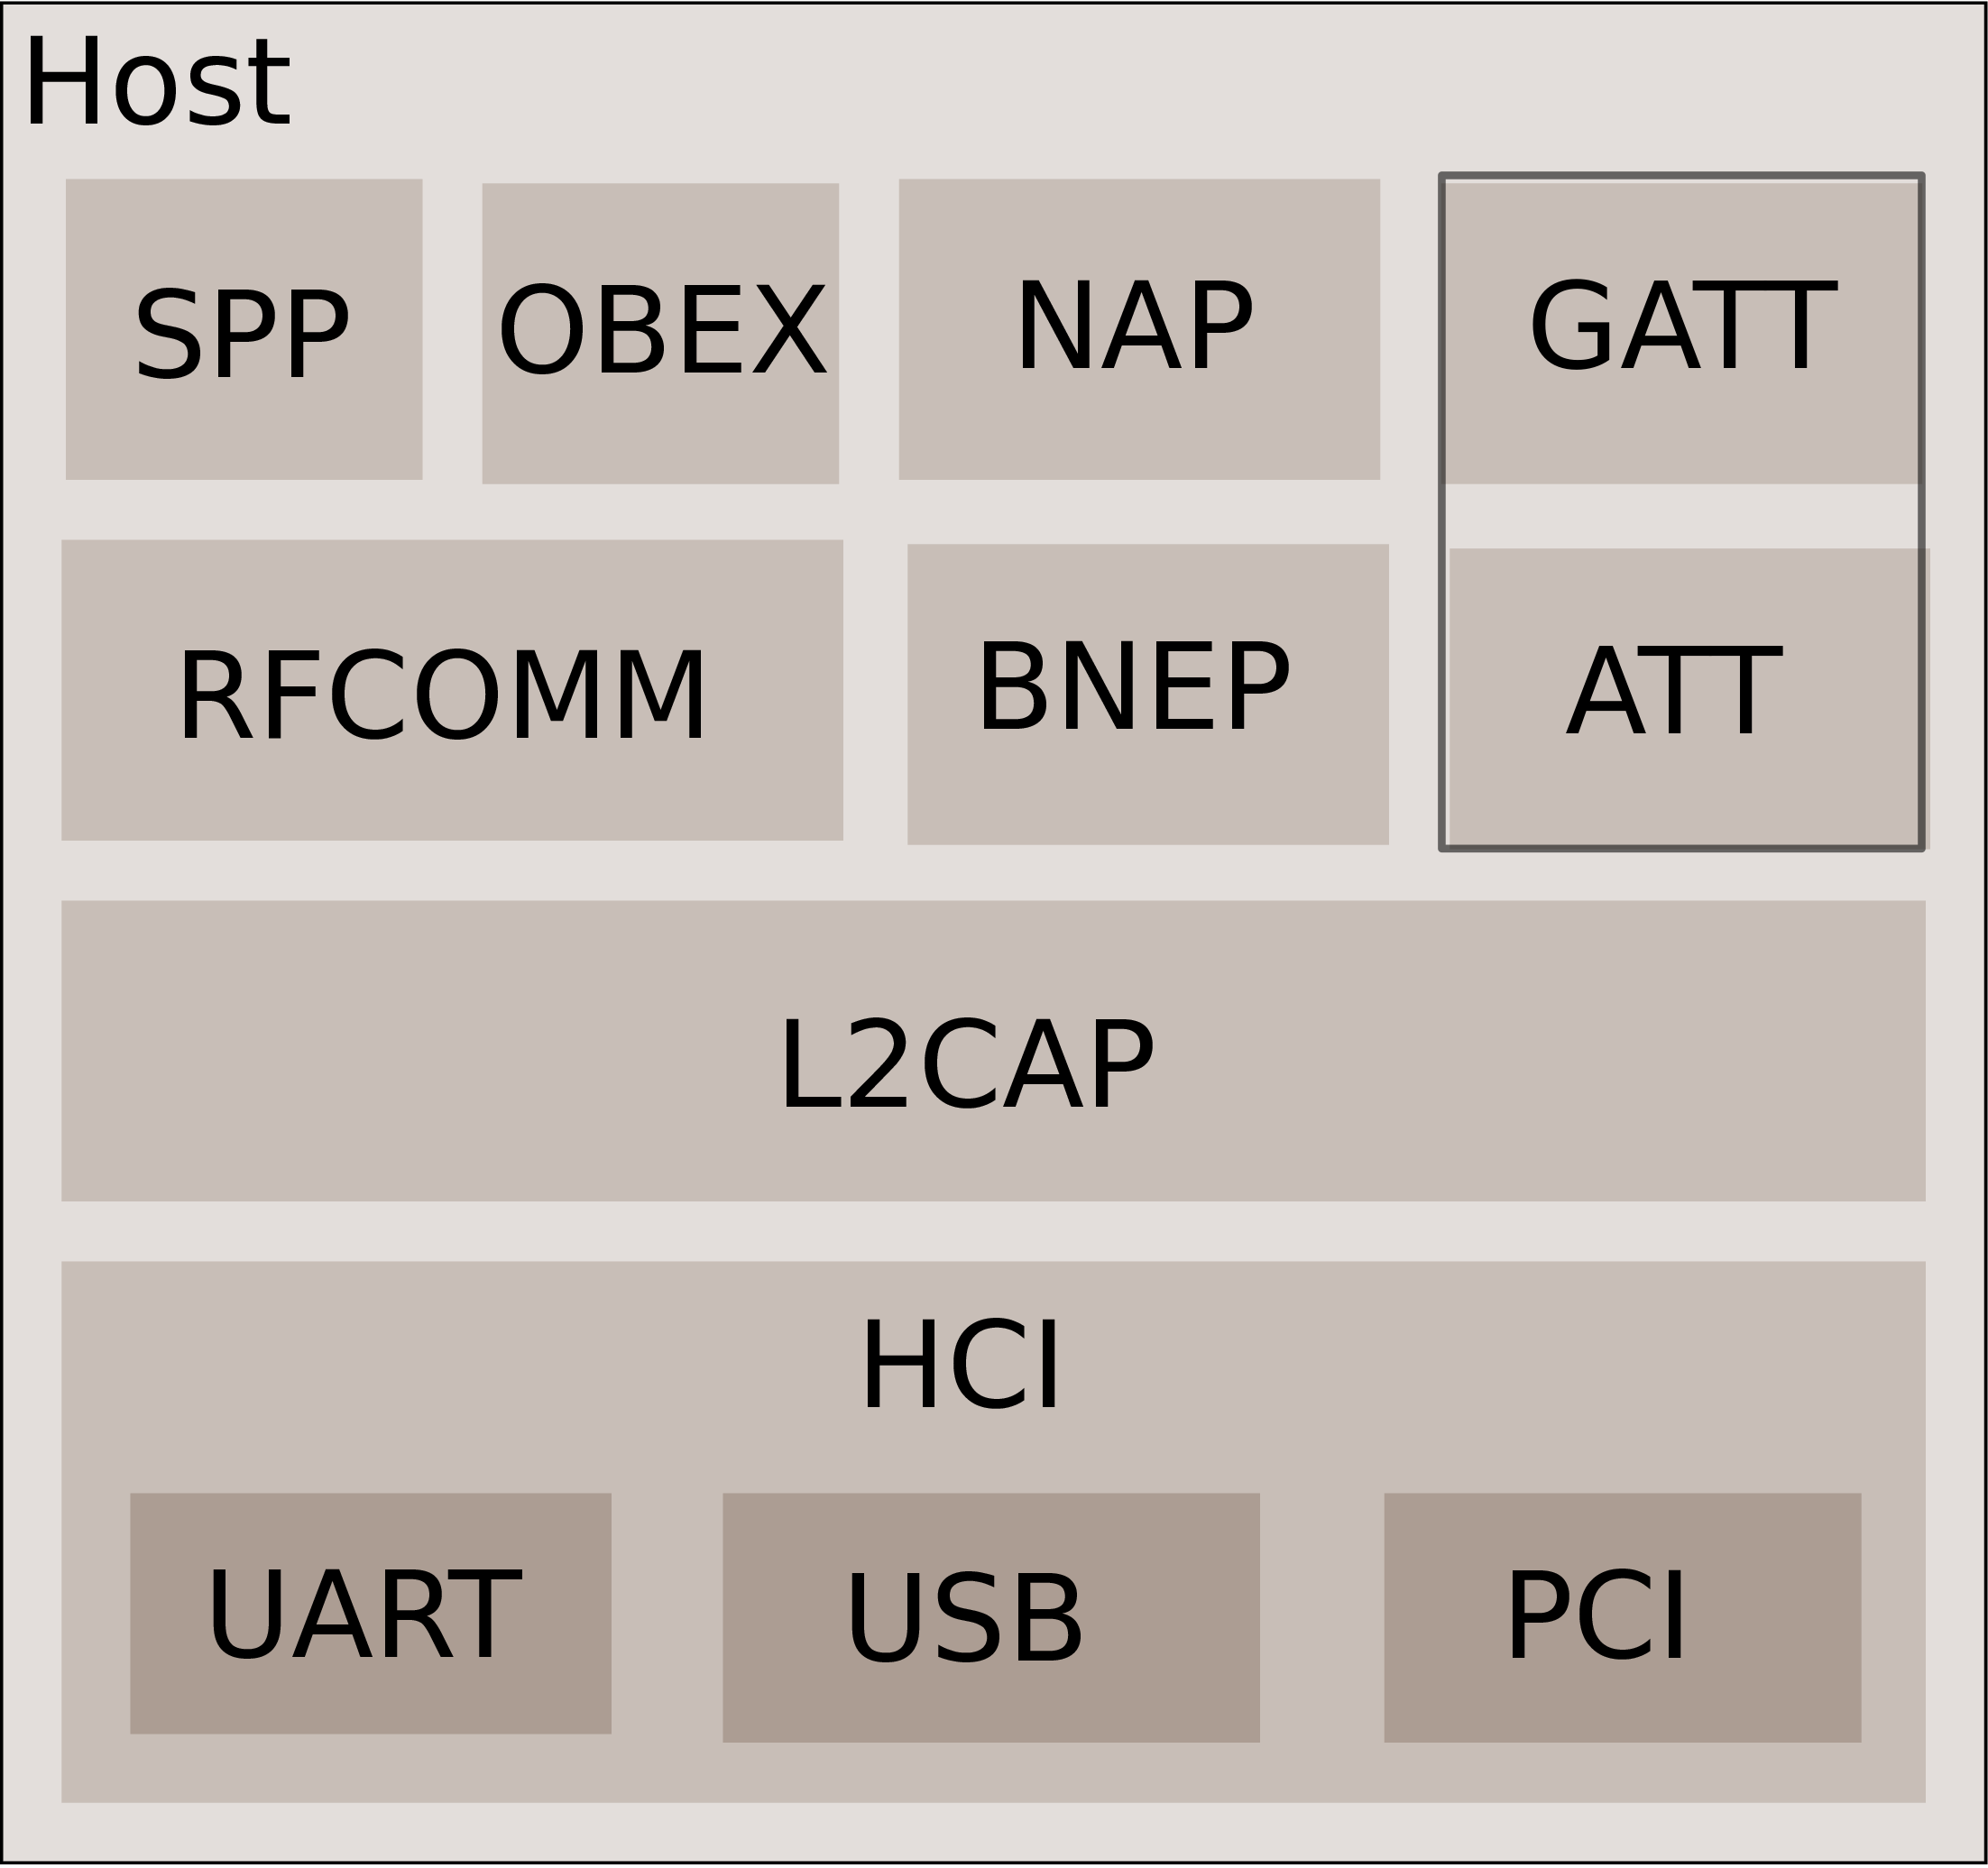
\includegraphics[height=5cm]{img/arch_log_all_ble.png}
				\caption{ATTributes / Generic ATTributes}
			\end{figure}
		}
	\end{minipage}
	\begin{minipage}[t]{0.38\linewidth}
		\uncover<2->{
		\begin{block}{ATT}
			\begin{itemize}
				\item Protocole
				\item Transport d'attributs
			\end{itemize}
		\end{block}
		}
		\uncover<3->{
		\begin{block}{GATT}
			Profil BLE
			\begin{itemize}
				\item Client
				\item Serveur
			\end{itemize}
		\end{block}
		}
	\end{minipage}
\end{frame}


\subsection{Attributs}
\begin{frame}
\begin{columns}[t]
\begin{column}{0.45\linewidth}
\begin{center} \huge GATT \end{center}
	\uncover<2->{
	\begin{block}{Attribut}
		\begin{itemize}
			\item Type : UUID
			\item Permissions : \begin{itemize}
						\item R/W
						\item Encryption
						\item Autorisation
					\end{itemize}
			\item Valeur
			\item Handle : Adresse
		\end{itemize}
	\end{block}
}
\end{column}
\begin{column}[t]{0.45\linewidth}
	\uncover<3->{
	\begin{block}{Services}
		\uncover<4->{
		Regroupe des :
		\begin{columns}[T]
		\begin{column}{0.90\textwidth}
		\begin{block}{Caractéristiques}
			\uncover<5->{
			\begin{itemize}
				\item Déclaration
				\item Valeur
				\item<6-> Et parfois :
			\end{itemize}
			\begin{columns}[T]
			\begin{column}{0.90\textwidth}
				\uncover<7->{
					\vspace{-0.5cm}
			\begin{block}{Descripteurs}
			Métadonnées sur la caractéristique
		}
			\end{block}
		}
			\end{column}
			\end{columns}
		\end{block}
		\end{column}
		\end{columns}
	}
	\end{block}
}
\end{column}
\end{columns}
\end{frame}

\begin{frame}
	\begin{figure}
		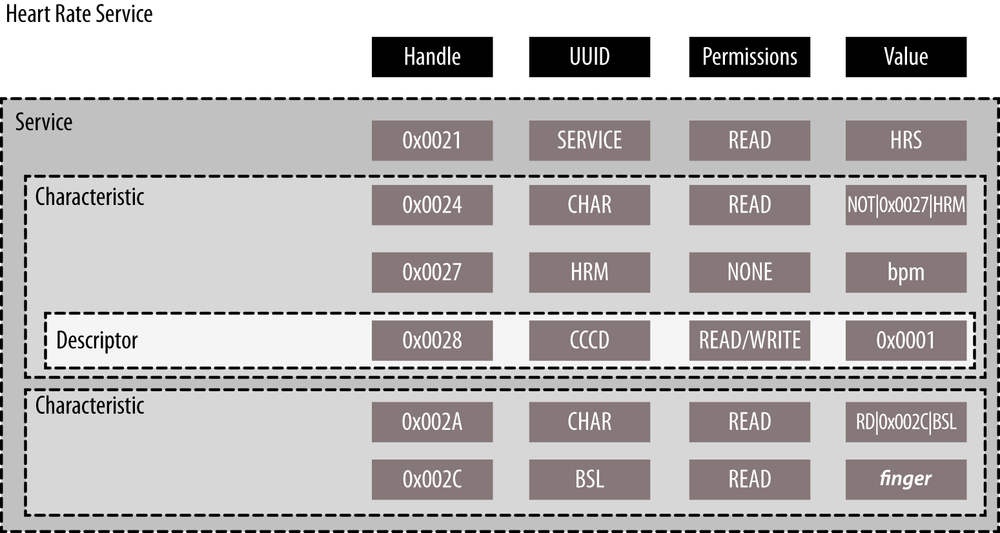
\includegraphics[height=5cm]{img/gatt.png}
		\caption{Exemple de service GATT}
	\end{figure}
{\tiny "Getting started with bluetooth low energy", R.Davidson, Akiba, Carles Cufí, Kevin Townsend, O'Reilly}
\end{frame}

\subsection{Bluez : Kernel}

%%%%%%%%%%%%%%%%%%%% HCI %%%%%%%%%%%%%%%%%%%%%%%%%%%%%%%
\begin{frame}
	\begin{columns}[t]
\begin{column}{0.60\linewidth}
	\begin{figure}
		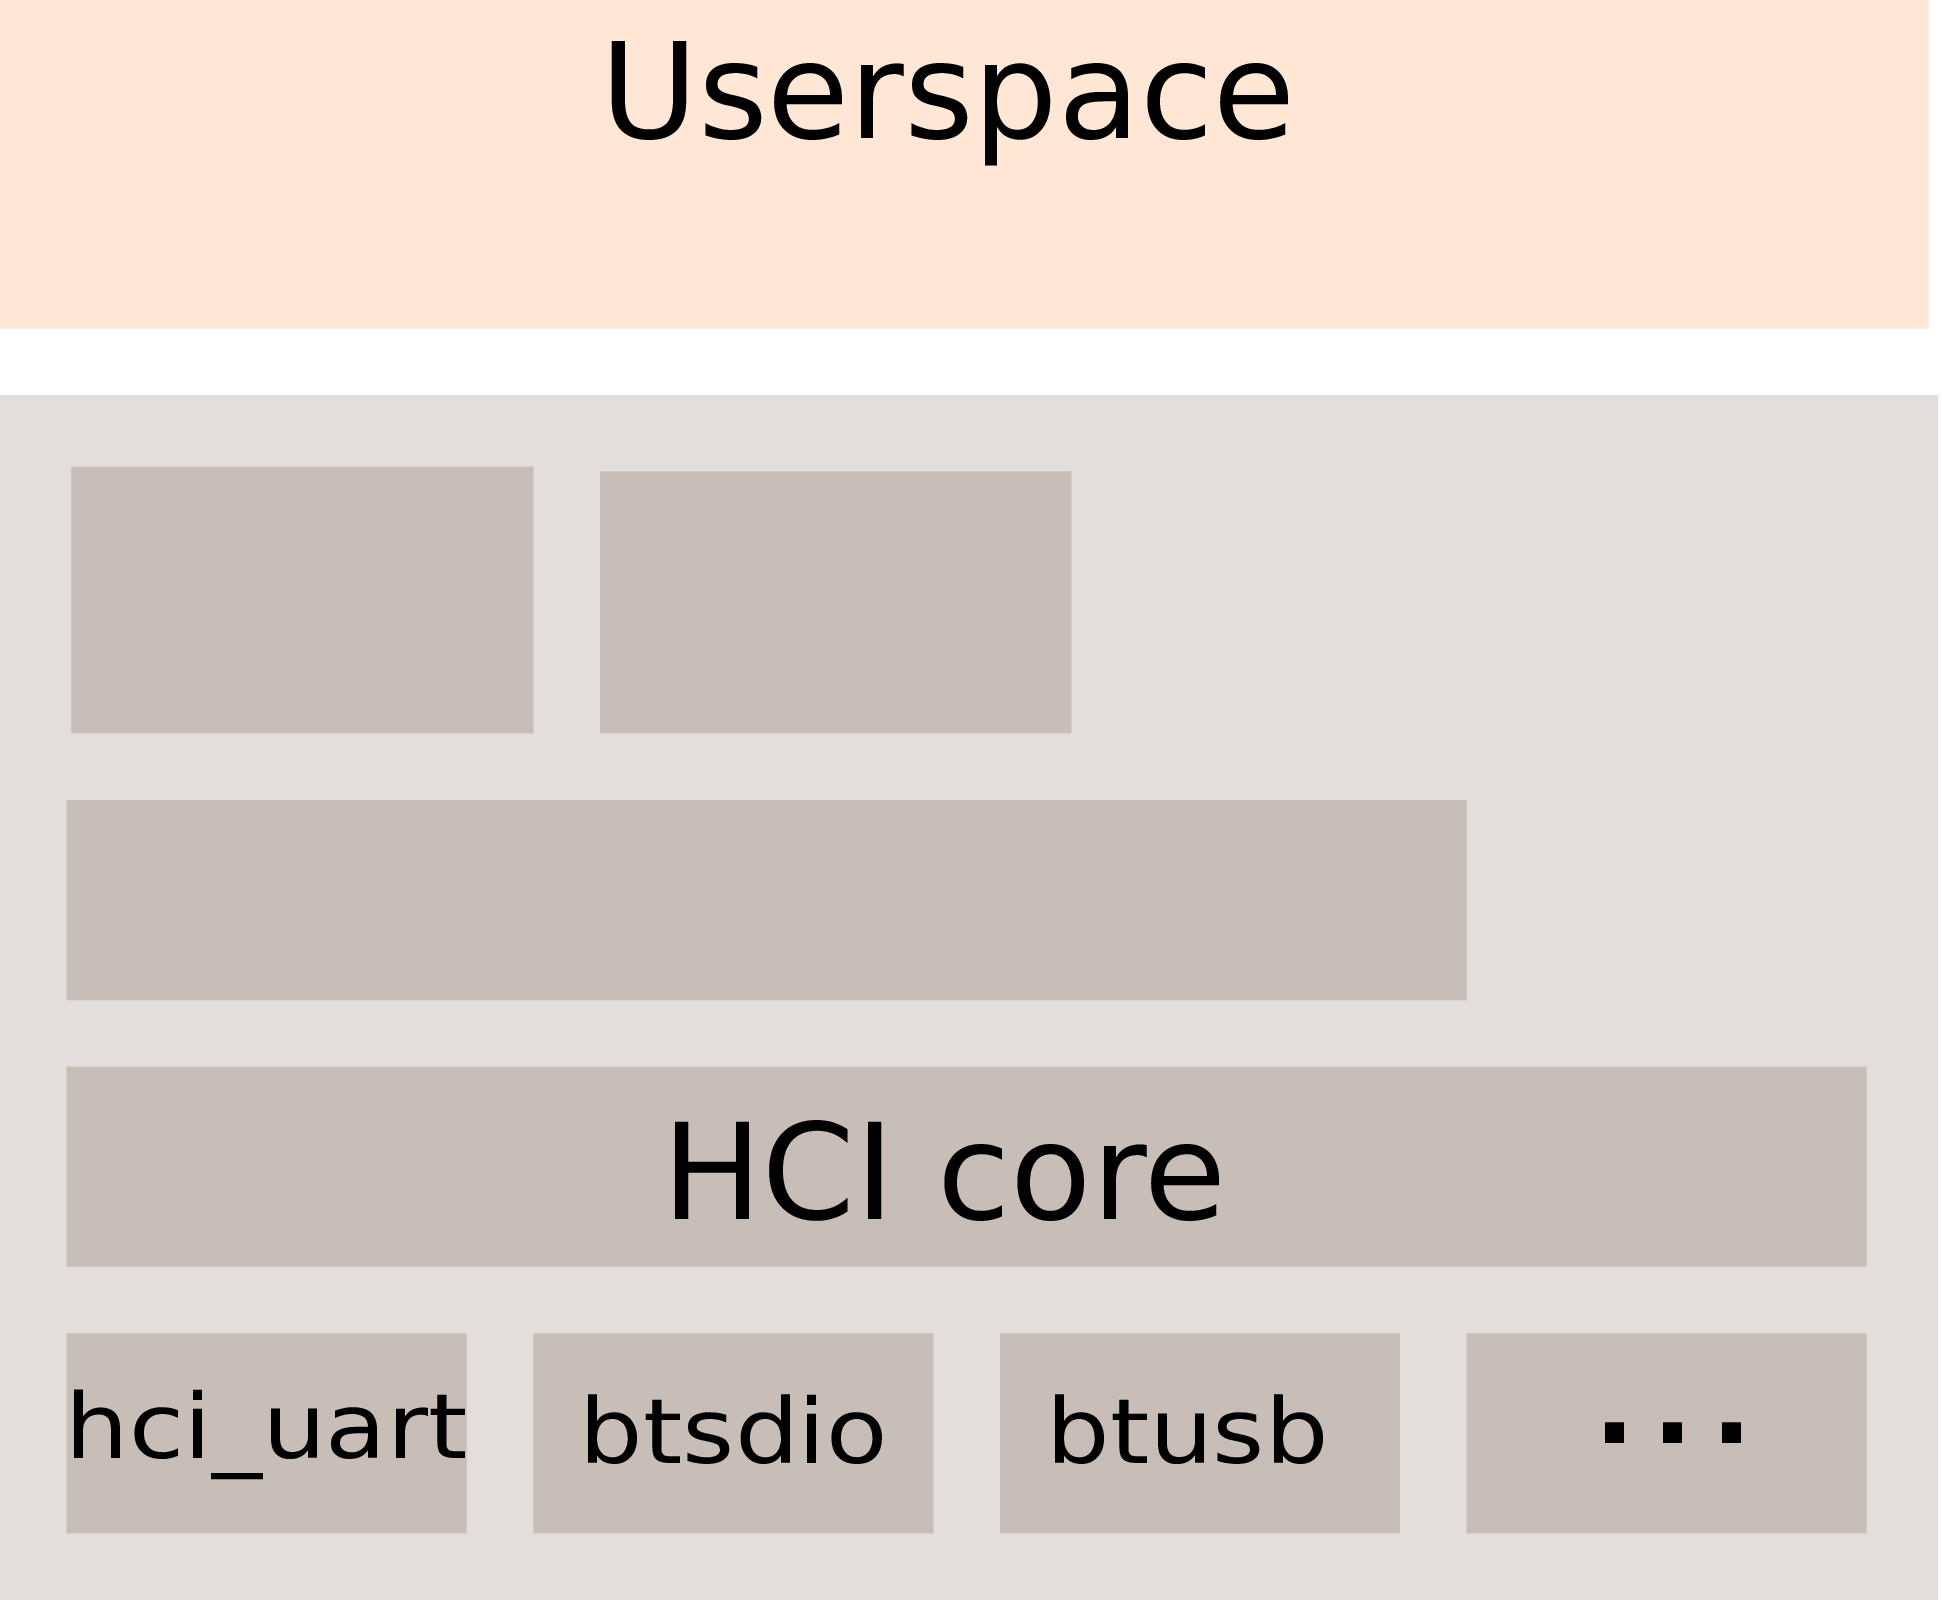
\includegraphics[height=5cm]{img/bluez_kernel_hci.png}
		\caption{Host to Controller Interface}
	\end{figure}
\end{column}
\begin{column}{0.40\linewidth}
	\begin{block}{HCI}
		\begin{itemize}
			\item Queueing
			\item Ordonnancement
		\end{itemize}
		Transport : 
		\begin{itemize}
			\item USB
			\item UART
			\item PCI
			\item SDIO
			\item PCMCIA
		\end{itemize}
	\end{block}
\end{column}
\end{columns}
\end{frame}

%%%%%%%%%%%%%%%%%%%% HCI MGMT %%%%%%%%%%%%%%%%%%%%%%%%%%%%%%%
\begin{frame}[fragile]
	\begin{columns}[t]
\begin{column}{0.60\linewidth}
	\begin{figure}
		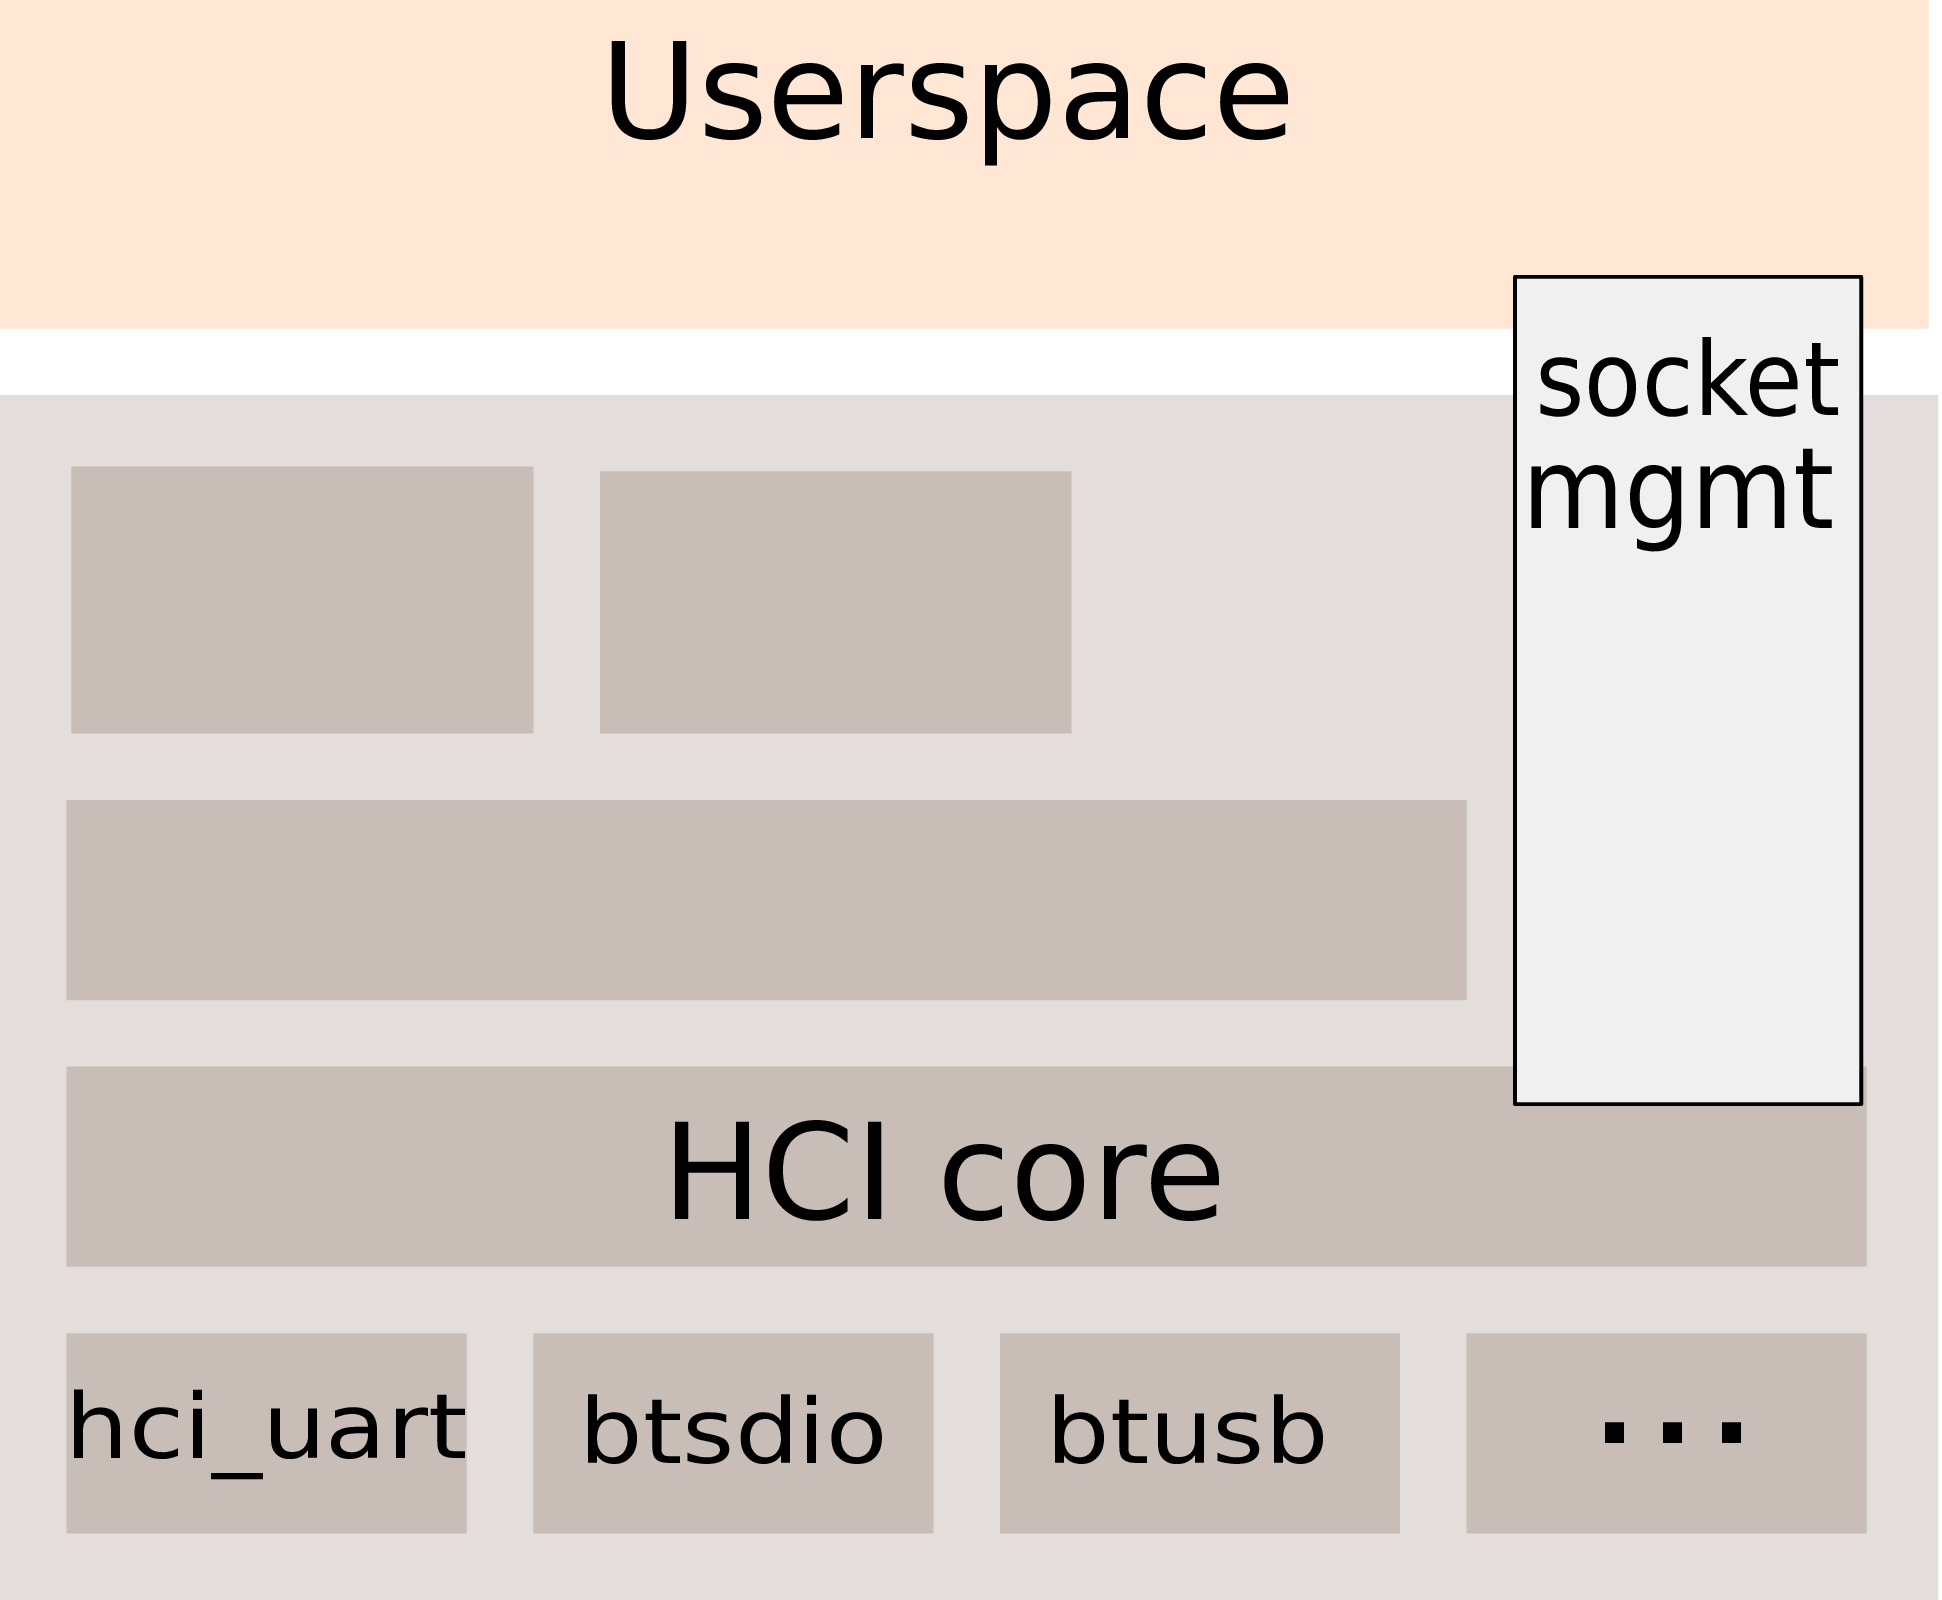
\includegraphics[height=5cm]{img/bluez_kernel_hci_sock.png}
		\caption{Management interface}
	\end{figure}
\end{column}
\begin{column}{0.40\linewidth}
	\begin{block}{mgmt socket}
		\begin{itemize}
			\item HCI pour userspace
			\item Remplace hci sockets
		\end{itemize}
	\end{block}
	\begin{block}{Paramètres}
		\begin{Verbatim}[fontsize=\tiny]
- PF_BLUETOOTH
- BTPROTO_HCI
struct sockaddr_hci
 - .hci_family = AF_BLUETOOTH
 - .hci_dev = HCI_DEV_NONE
 - .hci_channel = HCI_CHANNEL_CONTROL
		\end{Verbatim}
	\end{block}
\end{column}
\end{columns}
\end{frame}

%%%%%%%%%%%%%%%%%%%% L2CAP SOCKET %%%%%%%%%%%%%%%%%%%%%%%%%%%%%%%
\begin{frame}[fragile]
\begin{columns}[t]
\begin{column}{0.60\linewidth}
	\begin{figure}
		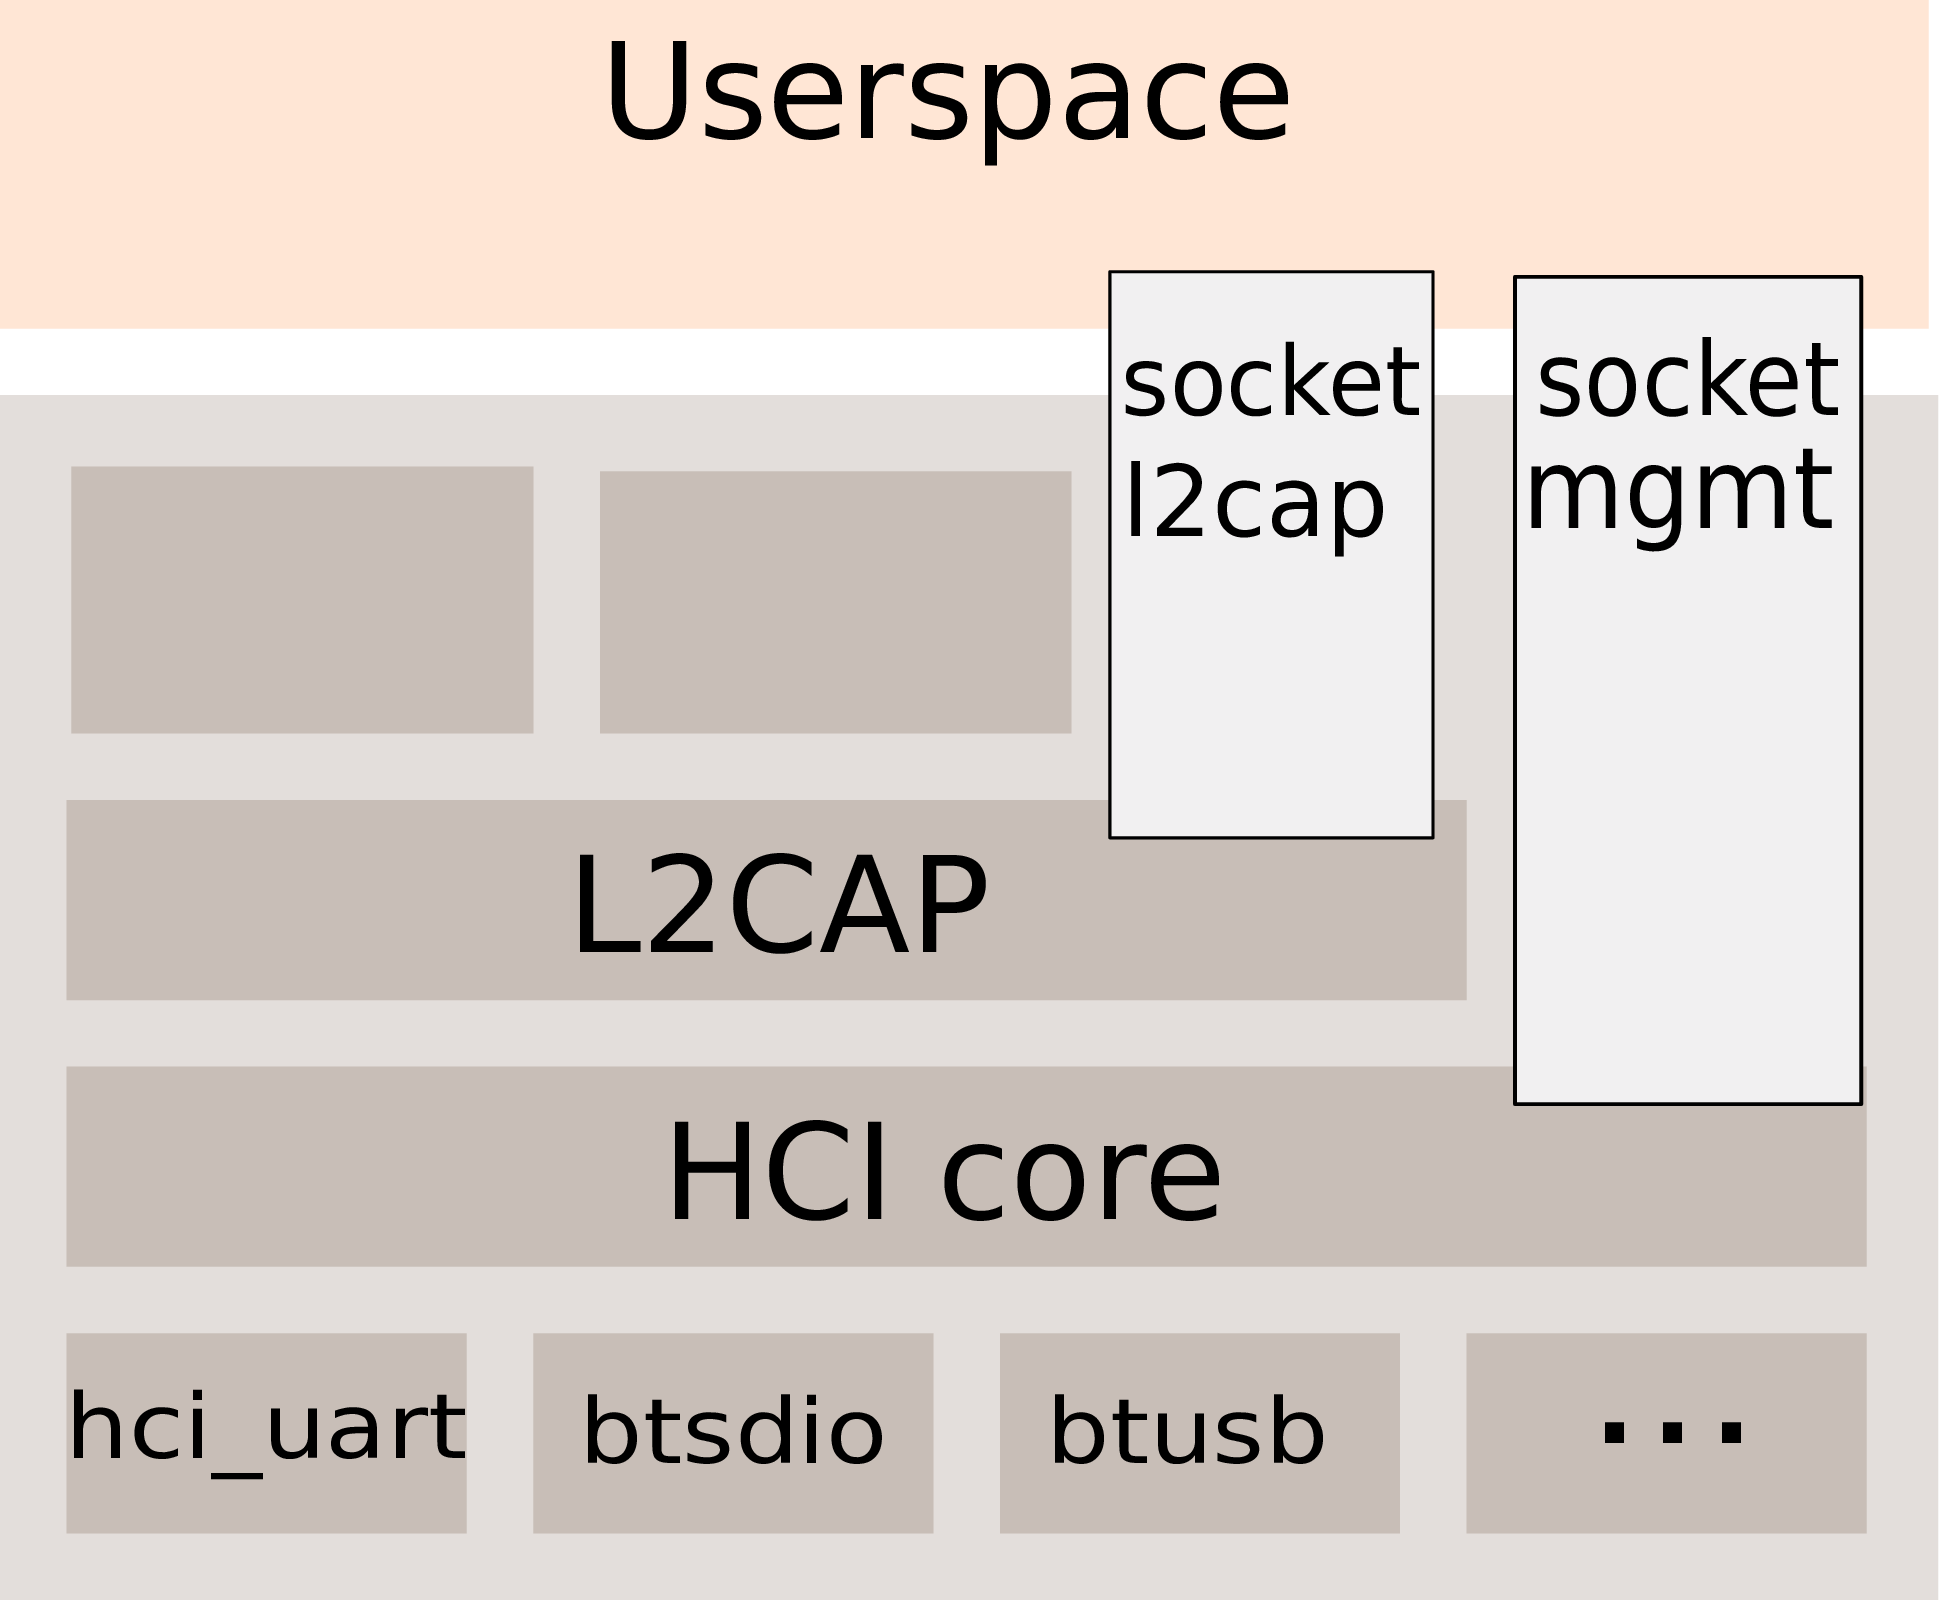
\includegraphics[height=5cm]{img/bluez_kernel_l2cap_sock.png}
		\caption{L2CAP}
	\end{figure}
\end{column}
\begin{column}{0.40\linewidth}
	\begin{block}{l2cap socket}
		\begin{itemize}
			\item API Socket
			\item - Adresse
			\item - PSM 
		\end{itemize}
	\end{block}
	\begin{block}{Paramètres}
		\begin{Verbatim}[fontsize=\tiny]
- AF_BLUETOOTH
- BTPROTO_L2CAP
struct sockaddr_l2
 - .l2_family = AF_BLUETOOTH
 - .l2_bdaddr = *BDADDR_ANY
 - .l2_psm = htobs(0x1001);
		\end{Verbatim}
	\end{block}
\end{column}
\end{columns}
\end{frame}

%%%%%%%%%%%%%%%%%%%% RFCOMM / BNEP SOCKET %%%%%%%%%%%%%%%%%%%%%%%%%%%%%%%
\begin{frame}[fragile]
\begin{columns}[t]
\begin{column}{0.60\linewidth}
	\begin{figure}
		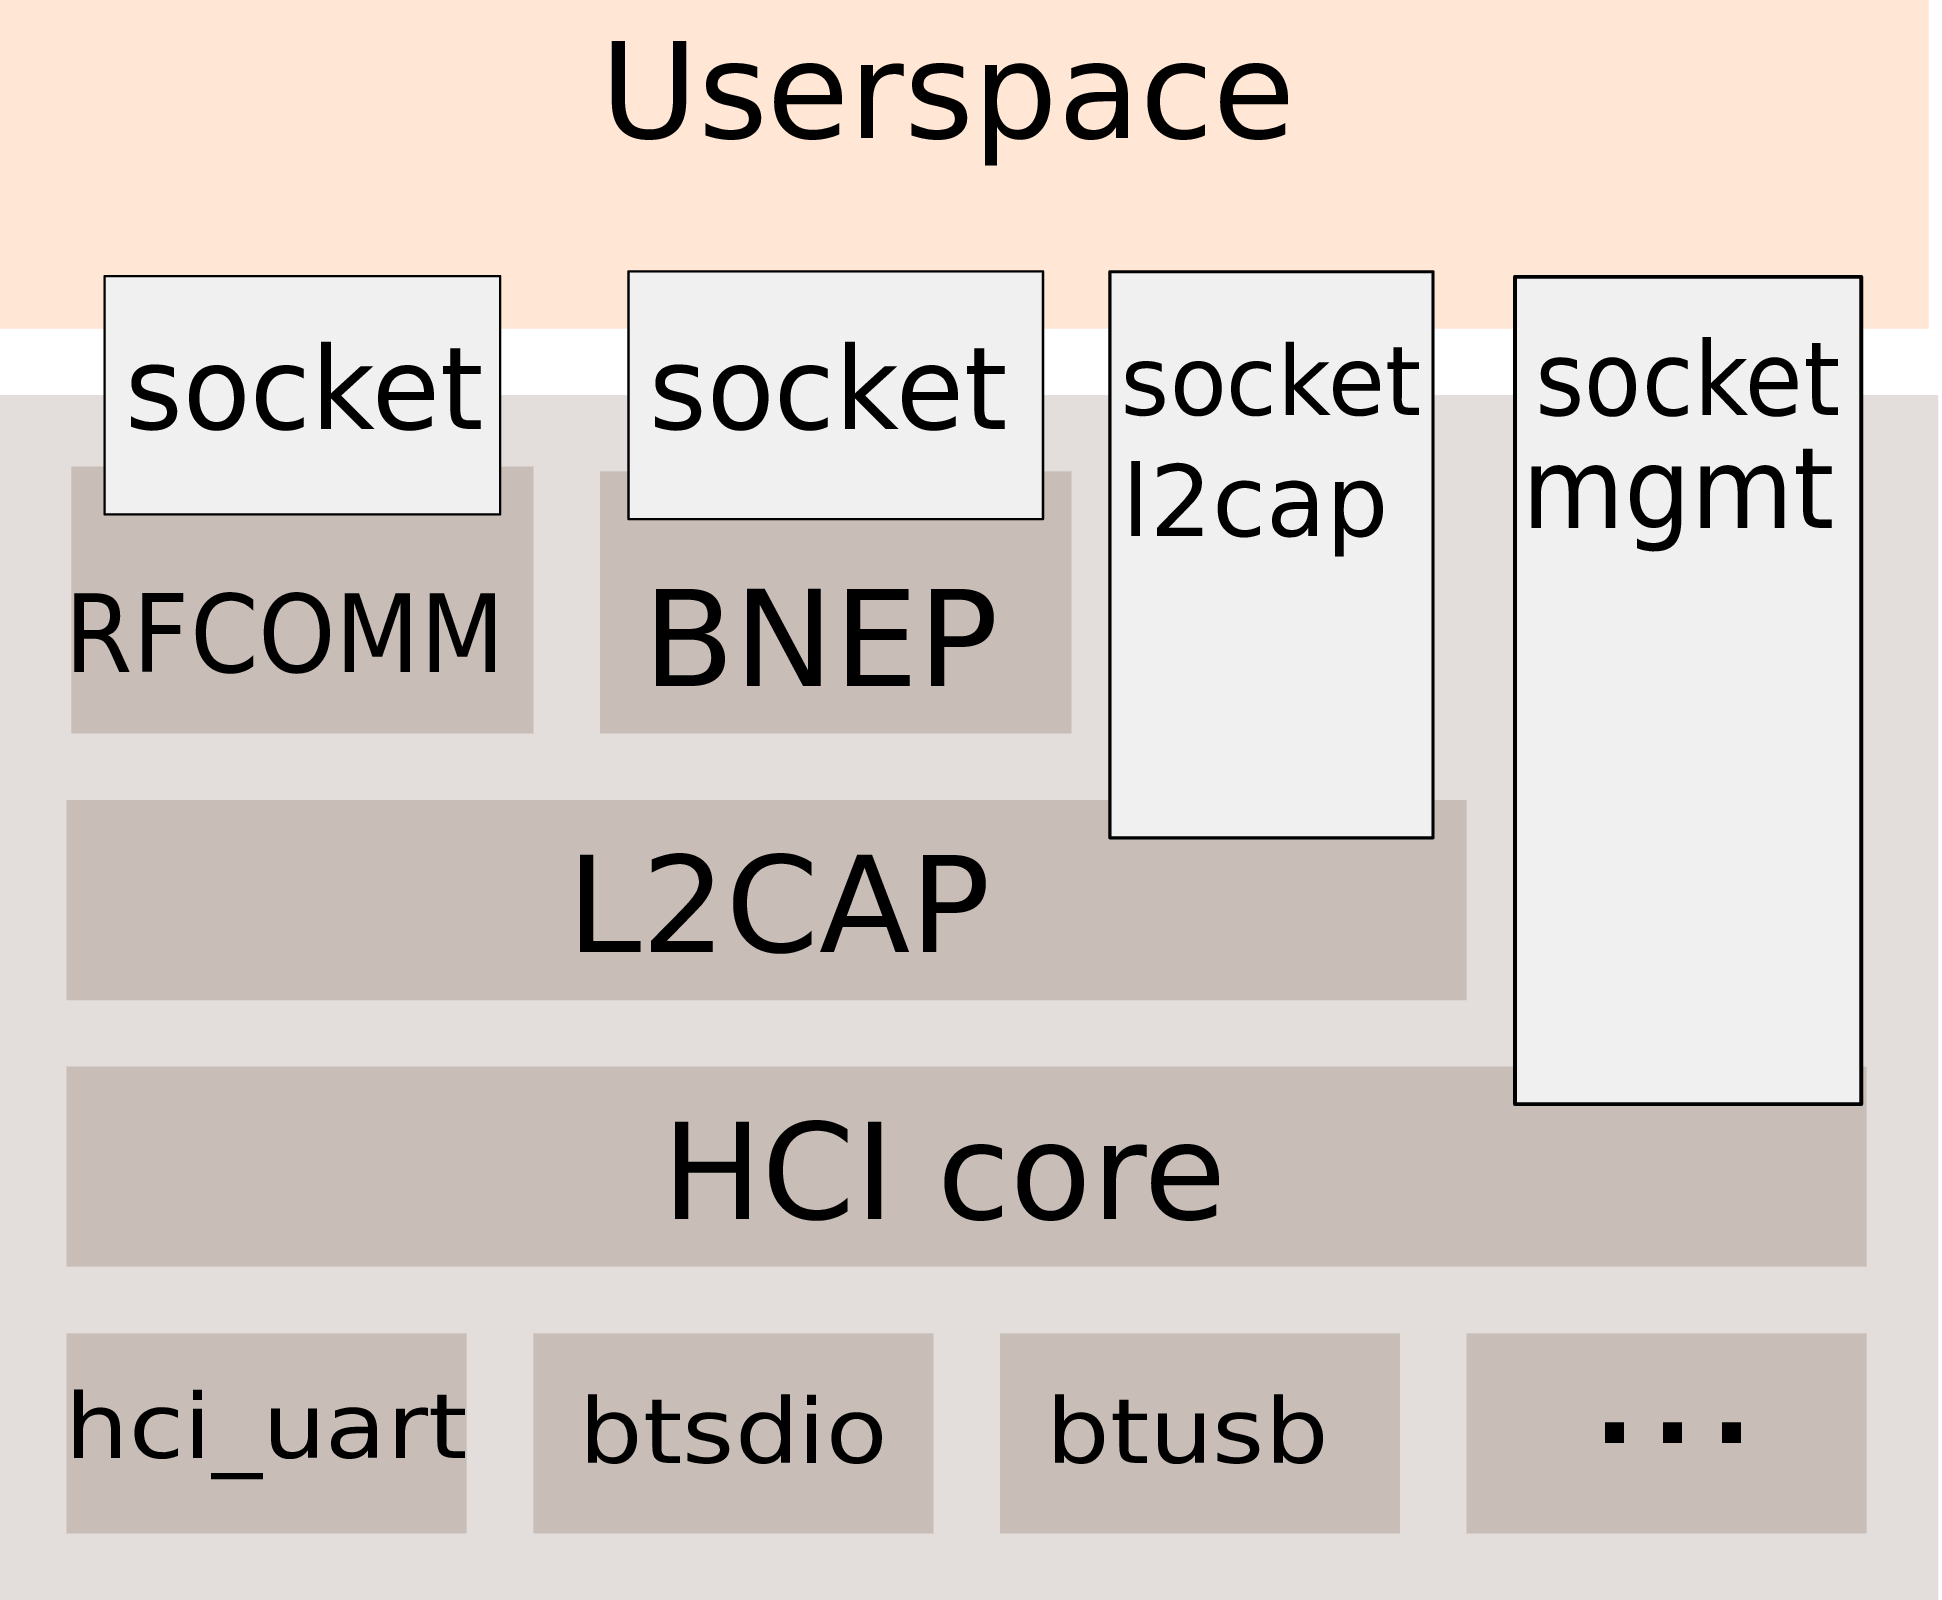
\includegraphics[height=5cm]{img/bluez_kernel.png}
		\caption{RFCOMM, BNEP, etc.}
	\end{figure}
\end{column}
\begin{column}{0.40\linewidth}
	\begin{block}{rfcomm socket}
		\begin{itemize}
			\item API Socket
			\item - Adresse
			\item - Canal
		\end{itemize}
	\end{block}
	\begin{block}{Paramètres}
		\begin{Verbatim}[fontsize=\tiny]
- AF_BLUETOOTH
- BTPROTO_RFCOMM
struct sockaddr_l2
 - .rc_family = AF_BLUETOOTH
 - .rc_channel = 1
 - .rc_braddr = *BRADDR_ANY;
		\end{Verbatim}
	\end{block}

\end{column}
\end{columns}
\end{frame}


\subsection{Bluez : Userspace}
\begin{frame}
\begin{minipage}[t]{0.60\linewidth}
	\begin{figure}
		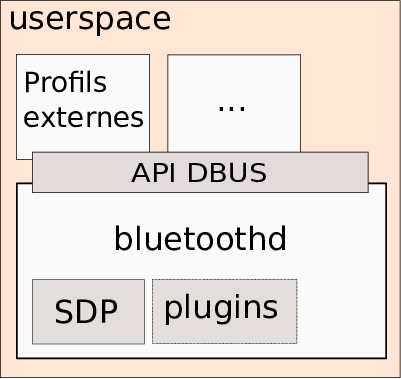
\includegraphics[height=9cm]{bluetoothd.png}
		\caption{bluetoothd}
	\end{figure}
\end{minipage}
\begin{minipage}[t]{0.30\linewidth}
	\begin{block}{Démon bluetoothd}
		\begin{itemize}
			\item Uniformisation
			\item Abstraction
		\end{itemize}
		Commandes : 
		\begin{itemize}
			\item Données
			\item Configuration
			\item Évènements
		\end{itemize}
	\end{block}
\end{minipage}
\end{frame}

\begin{frame}
	\begin{figure}
		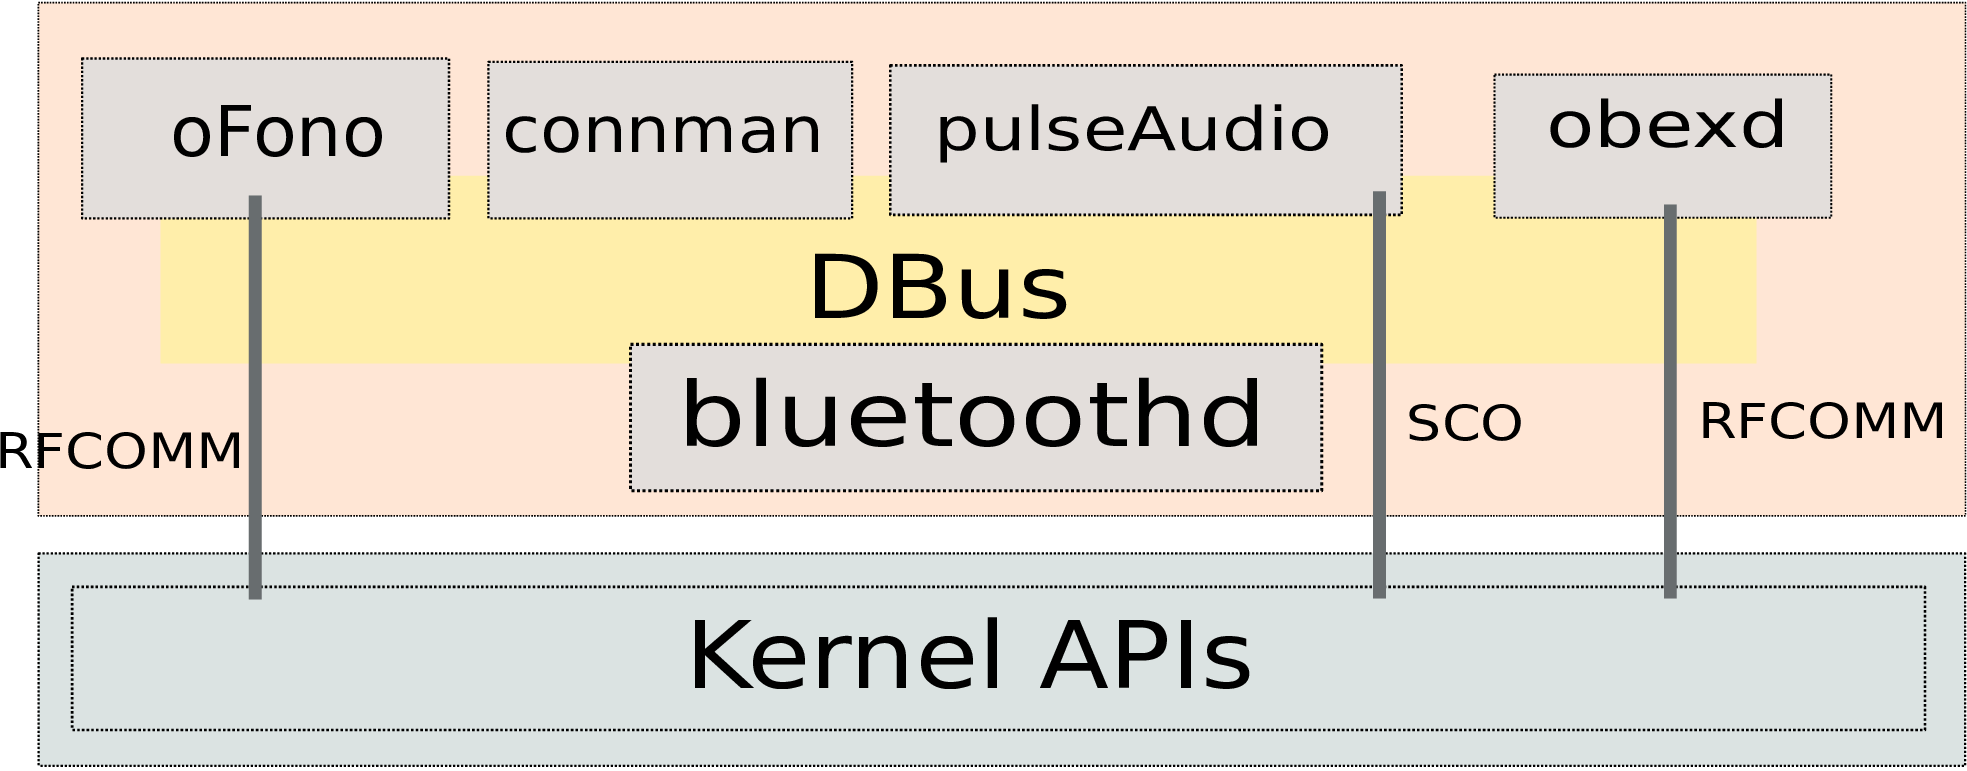
\includegraphics[height=3cm]{profiles_externes.png}
		\caption{Profils Externes}
	\end{figure}
	\begin{center}
\begin{columns}[t]
	\begin{column}{0.30\linewidth}
		\begin{block}{oFono}
			\begin{itemize}
				\item Gestion Téléphonie
				\item HFP / HSP
			\end{itemize}
		\end{block}
	\end{column}
	\begin{column}{0.30\linewidth}
		\begin{block}{connman}
			\begin{itemize}
				\item PAN ( NAP )
			\end{itemize}
		\end{block}
		\begin{block}{obexd}
			\begin{itemize}
				\item OBEX, OPP
			\end{itemize}
		\end{block}
	\end{column}
	\begin{column}{0.30\linewidth}
		\begin{block}{pulse audio}
			\begin{itemize}
				\item AD2P
				\item Gateway HFP
			\end{itemize}
		\end{block}
	\end{column}
\end{columns}
\end{center}
\end{frame}

\begin{frame}
\begin{center}\huge Outils\end{center}
	\begin{columns}[t]
		\begin{column}{0.50\linewidth}
			\begin{block}{bluetoothctl}
				\begin{itemize}
					\item Appairage
					\item SDP
				\end{itemize}
			\end{block}
			\begin{block}{obexctl}
				\begin{itemize}
					\item OBEX
					\item FTP
				\end{itemize}
			\end{block}
		\end{column}
		\begin{column}{0.50\linewidth}
			\begin{block}{btmgmt}
				\begin{itemize}
					\item mgmt API
					\item Low Energy config.
				\end{itemize}
			\end{block}
			\begin{block}{hcitool / hciconfig}
				\begin{itemize}
					\item HCI brut
				\end{itemize}
			\end{block}
		\end{column}
	\end{columns}
\end{frame}

\begin{frame}[fragile]
\begin{center}\huge Outils\end{center}
	\begin{columns}[t]
		\begin{column}{0.50\linewidth}
			\begin{block}{btmon}
			\end{block}
			\begin{block}{hcidump}
			\end{block}
		\end{column}
		\begin{column}{0.50\linewidth}
			\begin{itemize}
				\item \textbf{hciattach} \\ \verb+ hci over UART+
				\item \textbf{l2ping} \\ \verb+ test L2CAP+
				\item \textbf{rfcomm} \\ \verb+ gestion RFCOMM / SPP+
				\item \textbf{sdptool} \\ \verb+ gestion SDP+
			\end{itemize}
		\end{column}
	\end{columns}
\end{frame}


\begin{frame}
\begin{center}\huge Outils GATT\end{center}
	\begin{columns}[t]
		\begin{column}{0.50\linewidth}
			\begin{block}{btgatt-client}
			\end{block}
			\begin{block}{btgatt-server}
			\end{block}
		\end{column}
		\begin{column}{0.50\linewidth}
			\begin{block}{gatttool}
			\end{block}
		\end{column}
	\end{columns}
\end{frame}


\begin{frame}
API
\end{frame}




\end{document}
